\chapter{Experimental Setup and Results}\label{ch:4}
This chapter presents the empirical results that validate the decoupled, deep metric learning framework proposed in Chapter 3. Having detailed the systematic methodology, we now turn to the execution and outcomes of the multi-stage evaluation plan. The central objective of this chapter is to systematically assess the performance of each component of the pipeline---from the choice of embedding model and the impact of fine-tuning to the effects of dimensionality reduction and the selection of a downstream classifier---to identify the optimal configuration for both classification accuracy and computational efficiency.

The analysis is structured to first establish the validity of the core feature engineering approach before proceeding through the comparative stages of the evaluation. The chapter begins by detailing the computational environment, datasets, and formal evaluation metrics used throughout the experiments. It then immediately presents a critical ablation study to validate the efficacy of the novel composite distance vector (\(\Delta_c\)), the cornerstone of the feature representation. With the feature vector's design validated, the chapter then follows the primary evaluation sequence: first, establishing a baseline by assessing the performance of various off-the-shelf embedding models and classifiers; second, quantifying the performance gains achieved through fine-tuning; and third, analyzing the trade-offs between accuracy and efficiency introduced by dimensionality reduction. The chapter culminates in a definitive comparative analysis on the held-out test data, synthesizing all prior findings to identify the single best-performing pipeline configuration. We begin by outlining the experimental setup that forms the foundation for all subsequent results.

\section{Experimental Environment \& Datasets}
\subsection{Computational Environment}
The research presented in this thesis was conducted using a hybrid computational environment, leveraging both cloud-based services for initial language model evaluations and a powerful on-premise high-performance computing (HPC) cluster for the primary, computationally intensive experiments. The initial direct classification tasks described in Section 3.1 were performed using Google's Gemini v1.0, a proprietary cloud-based Large Language Model. All subsequent stages of the research, including model fine-tuning, embedding generation, dimensionality reduction, and the comprehensive downstream classifier evaluations, were executed on San Francisco State University's ``POLARIS'' High Performance Compute Cluster.

The POLARIS cluster provided a robust and flexible environment, running on Rocky Linux 8.9 with the Slurm Workload Manager for job scheduling. The GPU-intensive deep learning tasks, particularly the fine-tuning of the embedding models, were performed on the \verb|gpucluster| node. This node is equipped with two AMD EPYC 9334 CPUs (providing 64 cores and 128 threads), 1 TB of RAM, and is accelerated by four NVIDIA A100 GPUs, each with 80 GB of VRAM and supported by CUDA v12.4. The extensive hyperparameter grid searches for the traditional machine learning classifiers were primarily run on the \verb|cpucluster|, which consists of three nodes, each powered by two AMD EPYC 9534 CPUs (128 cores, 256 threads) and containing 576 GB of RAM. The cluster nodes are interconnected with a high-speed InfiniBand 200 Gb/s network, ensuring efficient data transfer during distributed tasks.

The entire experimental pipeline was implemented in Python, with Jupyter Notebooks serving as the primary environment for rapid prototyping, initial data exploration, and results analysis. The core deep learning components were built using PyTorch, with extensive use of the Hugging Face ecosystem, including the \verb|Transformers|, \verb|Sentence-Transformers|, and \verb|Hub| libraries for model access and training. The classical machine learning experiments were conducted using \verb|scikit-learn| and \verb|XGBoost|. Data manipulation and analysis were handled with \verb|numpy| and \verb|pandas|, while \verb|plotly| was used for visualization and \verb|dill| for object serialization.

\subsection{Datasets}
The evolutionary methodology described in Chapter~\ref{ch:3} was developed and validated using two distinct datasets, each serving a critical purpose at different stages of the research. The use of a smaller, initial dataset for prototyping followed by a larger, more comprehensive corpus for final evaluation is a core component of the experimental design. Table~\ref{tbl:datasets} provides a comparative summary of the key characteristics of both datasets used in this research.
\begin{table}[!tb]
    \captionsetup{skip=5pt}
    \centering
    \caption{Summary of Datasets Used in Evaluation}
    \label{tbl:datasets}
    \resizebox{\columnwidth}{!}{
        \begin{tabular}{p{0.2\textwidth} p{0.4\textwidth} p{0.4\textwidth}}
            \toprule
            \textbf{Characteristic} & \textbf{Initial Dataset}                                              & \textbf{PPM Corpus}                                  \\
            \midrule
            \textbf{Source}         & Manually curated via ASSIST                                           & Program Pathways Mapper (PPM)                        \\
            \addlinespace
            \textbf{Purpose}        & Preliminary screening, prototyping, and initial classifier evaluation & Definitive fine-tuning and final pipeline evaluation \\
            \addlinespace
            \textbf{Ground Truth}   & Established articulation agreements                                   & Course Identification Number (C-ID)                  \\
            \addlinespace
            \textbf{Final Size}     & 400 course pairs (for evaluation set)                                 & 2,157 courses (across 157 classes)                   \\
            \addlinespace
            \textbf{Partitioning}   & Stratified random sample                                              & Stratified 50/50 train/test split                    \\
            \bottomrule
        \end{tabular}
    }
\end{table}
\subsubsection{Initial Dataset}
The first dataset, hereafter referred to as the Initial Dataset, was a manually curated corpus used for the preliminary investigations in Stages 1 and 2 of the evaluation framework. This dataset was constructed from five lower-division courses at San Francisco State University and their established articulation agreements from 63 other California public colleges, sourced via the ASSIST repository. It was used to establish the initial performance baseline with the direct LLM classification approach and to prototype the decoupled pipeline. The final evaluation set for these preliminary stages consisted of a balanced, stratified random sample of 400 course pairs drawn from a larger set of over 11,000 generated pairs.

\subsubsection{PPM Corpus}
The primary and definitive experiments for this thesis were conducted on the PPM Corpus, a larger and more robust dataset provided by the Program Pathways Mapper (PPM). This corpus served as the foundation for the full-scale implementation, fine-tuning, and final validation of the decoupled pipeline (Stages 3 and 4). After a filtering process detailed in Section~\ref{ch:3.2.1}, the final corpus consists of 2,157 courses, each labeled with a Course Identification Number (C-ID) that serves as the ground truth for equivalency. This corpus was partitioned via a stratified 50/50 split into a training set of 1,078 courses and a held-out test set of 1,079 courses. This held-out test set is crucial for methodological rigor and was used only once for the final, conclusive evaluation of the optimized pipelines to provide an honest and unbiased estimate of their generalization performance.

\subsection{Evaluation Metrics}
To facilitate a comprehensive and multi-faceted analysis, a suite of standard evaluation metrics was used to assess the various pipeline configurations. These metrics were chosen to measure performance across two critical dimensions: classification efficacy and computational efficiency, ensuring that the final recommended pipeline is not only accurate but also practical for real-world deployment.

\subsubsection{Classification Efficacy}
The core assessment of classification performance is based on a standard suite of metrics derived from the confusion matrix, which tabulates the counts of True Positives (\(TP\)), True Negatives (\(TN\)), False Positives (\(FP\)), and False Negatives (\(FN\)). While Accuracy, defined as \(\frac{TP + TN}{TP + TN + FP + FN}\), provides a general overview of correctness, it can be insufficient for capturing the nuances of a classifier's behavior. Therefore, this research also evaluates:
\begin{itemize}
    \item \textbf{Precision}: Calculated as \(\frac{TP}{TP + FP}\), this metric measures a model's exactness. High precision indicates that when the model predicts an equivalency, it is likely to be correct.
    \item \textbf{Recall}: Calculated as \(\frac{TP}{TP + FN}\), this metric measures a model's completeness. High recall indicates that the model is effective at identifying the full set of all true equivalencies.
\end{itemize}
The \(F_1\)-Score, the harmonic mean of Precision and Recall (\(2\cdot\frac{Precision\cdot Recall}{Precision + Recall}\)), is used as the primary metric for reporting and comparing the final classification performance. The \(F_1\)-Score provides a single, robust value that balances the trade-off between precision and recall, making it an ideal metric for this task where both avoiding false equivalencies and identifying all true ones are important.

\subsubsection{Efficiency Metric}
Beyond classification efficacy, the practical viability of each pipeline was assessed by measuring its computational efficiency. Both Training Time and Inference Time were systematically captured during the hyperparameter tuning process using the detailed statistics provided by \verb|scikit-learn| \!\!'s \verb|GridSearchCV| utility. Training time reflects the resources required to fit a model configuration, offering insight into the cost of experimentation. Inference time, reported by \verb|GridSearchCV| as \verb|score_time|, measures the time required for a trained model to make predictions on new data. For the use case of this research, inference time is considered the more critical efficiency metric, as it directly impacts the system's real-world responsiveness and scalability in a production environment. Finally, for the specific task of monitoring model improvement during the fine-tuning process (Stage 3), a specialized metric, Average Precision based on cosine similarity, was employed by the \verb|BinaryClassificationEvaluator| to select the best-performing model checkpoint.

\section{Direct LLM Classification}
The initial phase of this research sought to establish a performance baseline by evaluating the feasibility of using a Large Language Model for end-to-end course equivalency classification. The experiments were conducted using the Initial Dataset, a balanced 400-pair sample, and leveraged Google's Gemini Pro v1.0 as the reasoning engine. The evaluation was designed to test two key conditions: the impact of input data type (full raw text vs.\ extracted topics) and the effect of different classification schemes (binary, 3-way, and 4-way) on the model's performance and behavior.

The classification results were encouraging, with the model achieving a peak accuracy of 90.5\% in the binary task using raw text. A primary finding from this phase was that using the full, unprocessed raw text consistently yielded superior results compared to using only the extracted structured topics. This performance gap is likely attributable to the challenges inherent in the data extraction step itself. The process of deducing structured topics from unstructured text proved to be the most time-consuming and difficult aspect of this initial approach, requiring two to four times more time than the classification task and exhibiting a high sensitivity to prompt wording—a finding that aligns with previous studies on prompt engineering by Sclar et al., Errica et al., Chen et al., Cheung, and Gerych et al.~\cite{Sclar2023QuantifyingLM,Errica2024WhatDI,Chen2024LLMAA,Cheung2024ARC,Gerych2024WhoKT}. Although Gemini demonstrated a general capability to understand the context of the course descriptions, its limitations in flawlessly deducing course topics appear to have introduced enough noise to degrade the performance of the topics-based classification.

An analysis of the confusion matrices, presented in Figure~\ref{fig:cm} reveals a consistent and telling behavioral pattern: the model exhibits a strong conservative bias. Across all scenarios, the ``not equivalent'' class showed higher recall than precision, while the ``equivalent'' class showed higher precision than recall. For example, in the binary raw text evaluation, the model produced 34 false negatives but only 4 false positives. This indicates that the model is far more likely to misclassify a truly equivalent course as ``not equivalent'' than it is to incorrectly approve a non-equivalent pair. This conservative tendency suggests the LLM operates with a high internal threshold for declaring equivalency, preferring to err on the side of caution.
\begin{figure}[tb]
    \captionsetup{skip=5pt}
    \centering
    \begin{subfigure}[b]{0.497\textwidth}
        \centering
        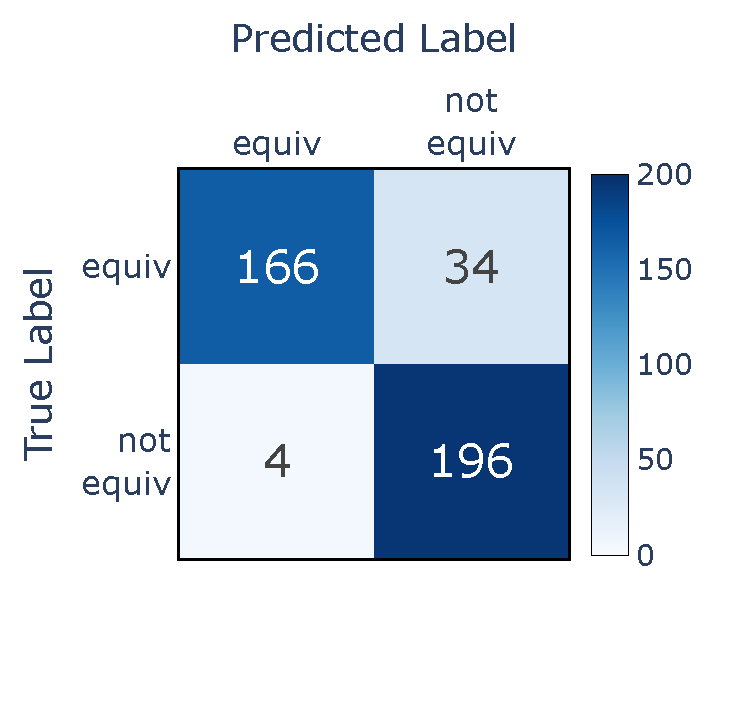
\includegraphics[scale=0.395,trim={3mm 20mm 7mm 0},clip]{LLMeval_binary_raw_text_cm.pdf}
        \caption{Binary Raw Text}
        \label{fig:sub_brt}
    \end{subfigure}
    \hfill
    \begin{subfigure}[b]{0.497\textwidth}
        \centering
        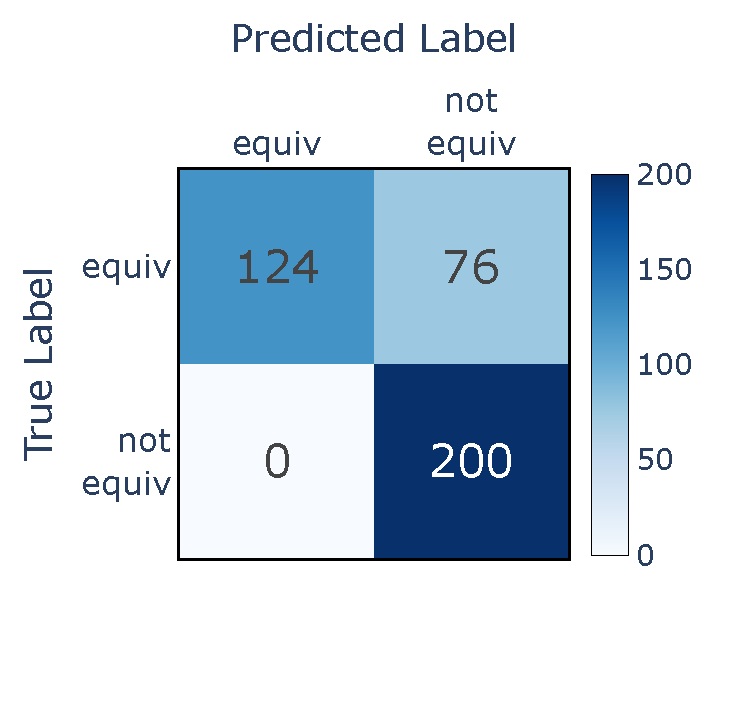
\includegraphics[scale=0.42,trim={3mm 20mm 7mm 0},clip]{LLMeval_binary_topics_cm.pdf}
        \caption{Binary Topics}
        \label{fig:sub_brt}
    \end{subfigure}

    \vspace{2mm}

    \begin{subfigure}[b]{0.497\textwidth}
        \centering
        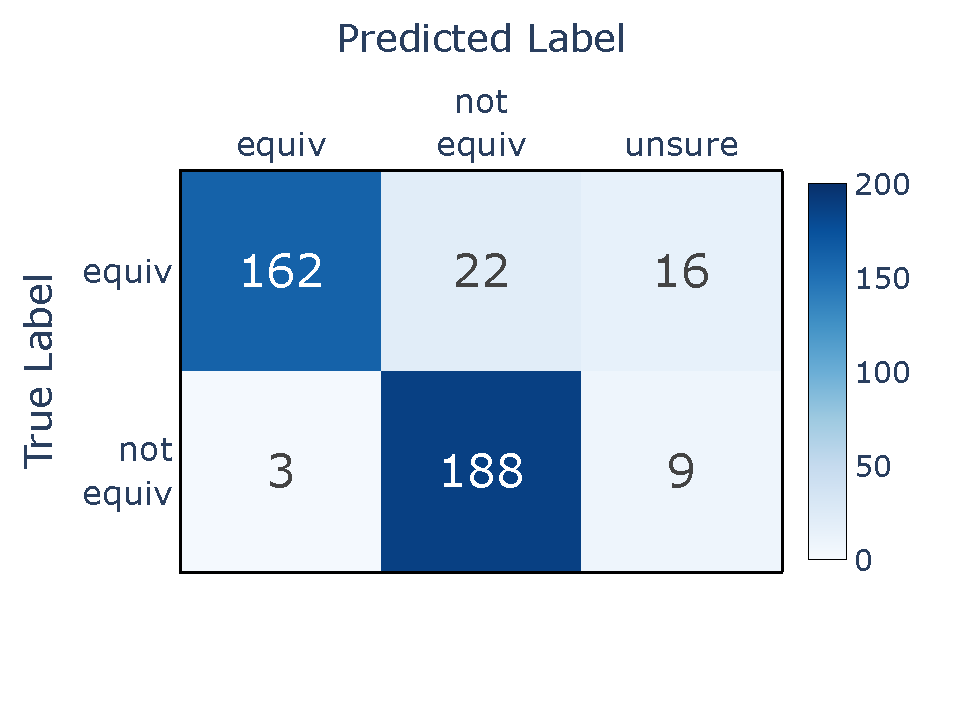
\includegraphics[scale=0.42,trim={3mm 20mm 7mm 0},clip]{LLMeval_3way_raw_text_cm.pdf}
        \caption{3-way Raw Text}
        \label{fig:sub_brt}
    \end{subfigure}
    \hfill
    \begin{subfigure}[b]{0.497\textwidth}
        \centering
        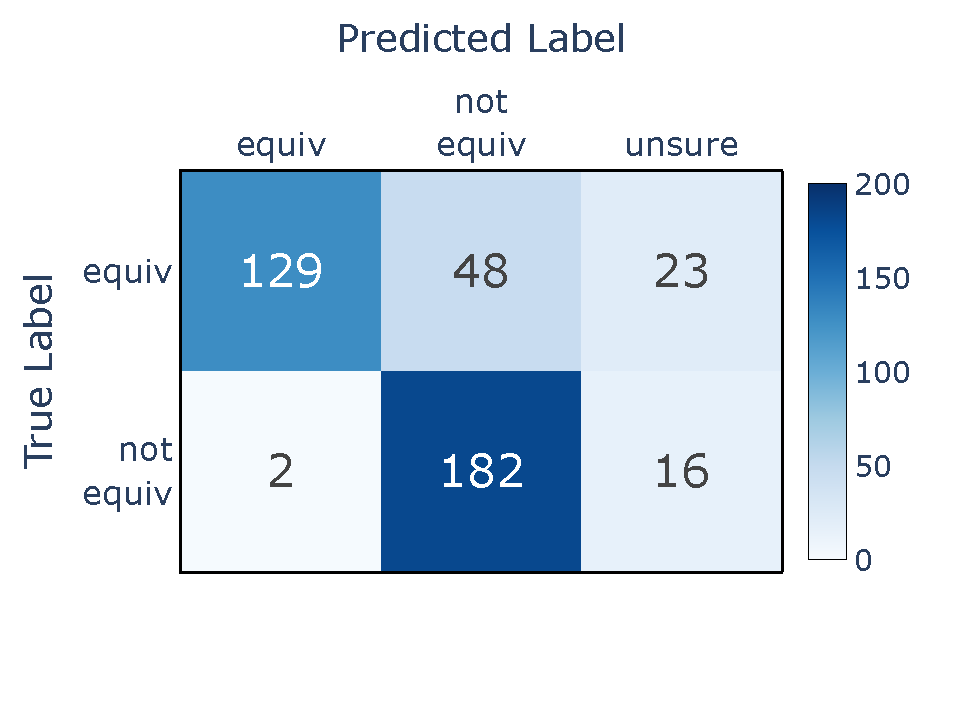
\includegraphics[scale=0.42,trim={3mm 20mm 7mm 0},clip]{LLMeval_3way_topics_cm.pdf}
        \caption{3-way Topics}
        \label{fig:sub_brt}
    \end{subfigure}

    \vspace{2mm}

    \begin{subfigure}[b]{0.497\textwidth}
        \centering
        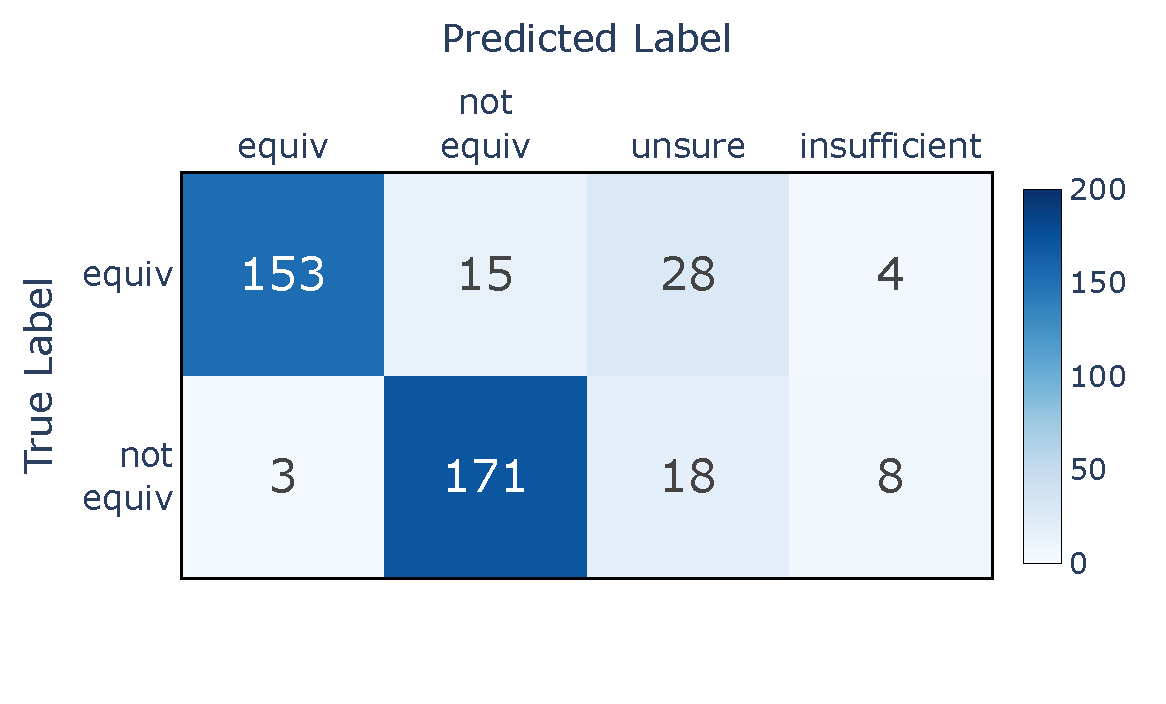
\includegraphics[scale=0.42,trim={3mm 20mm 7mm 0},clip]{LLMeval_4way_raw_text_cm.pdf}
        \caption{4-way Raw Text}
        \label{fig:sub_brt}
    \end{subfigure}
    \hfill
    \begin{subfigure}[b]{0.497\textwidth}
        \centering
        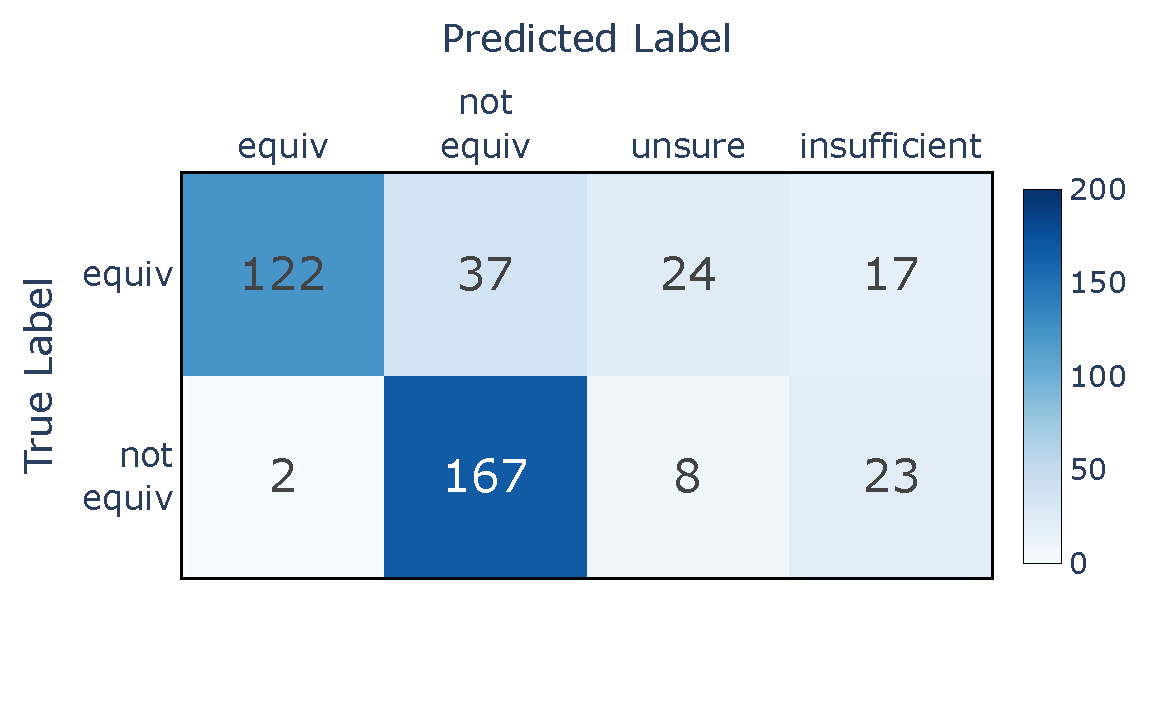
\includegraphics[scale=0.42,trim={3mm 20mm 7mm 0},clip]{LLMeval_4way_topics_cm.pdf}
        \caption{4-way Topics}
        \label{fig:sub_brt}
    \end{subfigure}
    \caption{LLM Classification Confusion Matrices}
    % {\footnotesize Clockwise from bottom left: 4-class raw text, 3-class raw text, binary raw text, binary
    %     structured topics, 3-class structured topics, and 4-class structured topics.\\\footnotemark[1]ins: insufficient description}
    \label{fig:cm}
\end{figure}

The introduction of the ``unsure'' and ``insufficient data'' categories was designed to simulate how a human advisor might handle ambiguity. While there is no ground truth for these labels, their value lies in the model's ability to isolate cases that require further manual review. This is particularly relevant for courses that may have significant topical overlap but different learning outcomes, or for descriptions that are too sparse to allow for a definitive decision. For instance, in the 4-way raw text evaluation, the model flagged 46 pairs as ``unsure'' and 12 as having ``insufficient'' information, effectively separating these ambiguous cases from the main classification flow.  Table~\ref{tbl:llm_results_summary} provides a comprehensive summary of the performance metrics for all six experimental conditions.
\begin{table}[!tb]
    \captionsetup{skip=5pt}
    \centering
    \caption{Performance Summary of Direct LLM Classification}
    \label{tbl:llm_results_summary}
    \begin{tabular}{lccccc}
        \toprule
                                  & \textbf{Classification} &                   &                    &                     &                   \\
        \textbf{Input Data}       & \textbf{Task}           & \textbf{Accuracy} & \textbf{F1-Score*} & \textbf{Precision*} & \textbf{Recall*}  \\
        \midrule
        \multirow{3}{*}{Raw Text} & Binary                  & 0.9050            & 0.8973             & 0.9765              & 0.8300            \\
                                  & 3-way                   & 0.8750            & 0.8877             & 0.9818              & 0.8100            \\
                                  & 4-way                   & 0.8100            & 0.8596             & 0.9808              & 0.7650            \\
        \midrule
        \multirow{3}{*}{Topics}   & Binary                  & 0.8100            & 0.7654             & 1.0000              & 0.6200            \\
                                  & 3-way                   & 0.7775            & 0.7795             & 0.9847              & 0.6450            \\
                                  & 4-way                   & 0.7225            & 0.7531             & 0.9839              & 0.6100            \\
        \bottomrule
        \multicolumn{6}{p{0.9\textwidth}}{\scriptsize * F1-Score, Precision, and Recall are reported for the positive class (``Equivalent'').} \\
    \end{tabular}
\end{table}

To contextualize the performance of Gemini Pro, a comparative analysis was conducted against a suite of other prominent open-source LLMs (see Table~\ref{tbl:cls} for a summary of their specifications and performance). The results of this benchmark revealed that Gemini Pro v1.0 outperformed all other models tested. While most models were able to complete the task, their performance varied significantly. The strongest competitor was Anthracite Magnum v1 72B, which achieved a respectable accuracy of 85.25\%, but still falling short of Gemini's 90.5\%.
\begin{table}[tb]
    \captionsetup{skip=5pt}
    \caption{Model Specifications and Performance}
    \label{tbl:cls}
    \centering
    \resizebox{\columnwidth}{!}{
        \begin{tabular}{lccccccc}
            \toprule
                                            &                      & \textbf{Context}                &                  &                   &
                                            &                      &                                                                                                                     \\
            \textbf{Model Name}             & \textbf{Parameters*} & \textbf{Length}                 & \textbf{Support} & \textbf{Accuracy} &
            \textbf{Precision}              & \textbf{Recall}      & \(\mathbf{F_1}\)\textbf{-score}                                                                                     \\
            \midrule
            Google Gemini Pro 1.0           & Unknown              & 32,768                          & 400              & \textbf{0.9050}   & 0.9765 & \textbf{0.8300} & \textbf{0.8973} \\
            Meta Llama 3.1 8B Instruct      & 8                    & 128,000                         & 208 (52\%)       & 0.6250            & 1.0000 & 0.3500          & 0.5185          \\
            Microsoft Phi 3 Medium Instruct & 14                   & 128,000                         & 400              & 0.7100            & 1.0000 & 0.4200          & 0.5915          \\
            Google Gemma 2 27b              & 27.2                 & 8,000                           & N/A              & N/A               & N/A    & N/A             & N/A             \\
            Meta Llama 3.1 70B Instruct     & 70                   & 128,000                         & 400              & 0.7350            & 1.0000 & 0.4700          & 0.6395          \\
            Qwen 2 72B Instruct             & 72.7                 & 131,072                         & 400              & 0.7650            & 1.0000 & 0.5300          & 0.6928          \\
            Anthracite Magnum v1 72B        & 72.7                 & 32,768                          & 400              & 0.8525            & 1.0000 & 0.7050          & 0.8270          \\
            CalmeRys 78B Orpo v0.1          & 78                   & 32,768                          & 400              & 0.7175            & 1.0000 & 0.4350          & 0.6063          \\
            Mixtral 8x22B Instruct v0.1     & 141                  & 65,536                          & 400              & 0.6450            & 1.0000 & 0.2900          & 0.4496          \\
            Meta Llama 3.1 405B Instruct**  & 405                  & 128,000                         & 400              & 0.7775            & 1.0000 & 0.5550          & 0.7138          \\
            \bottomrule
            \multicolumn{8}{l}{\footnotesize *in Billions}                                                                                                                               \\
            \multicolumn{8}{l}{\footnotesize **INT4 Quantized Model}
        \end{tabular}
    }
\end{table}

This benchmark also highlighted significant operational challenges. Several models struggled to reliably produce valid output. For example, Google's Gemma 2 27B consistently generated unintelligible or irrelevant responses, preventing the collection of any meaningful performance data. Similarly, Meta's Llama 3.1 8B Instruct model was only able to respond correctly to approximately 52\% of the prompts, making it too unreliable for practical use. A surprising insight from this analysis was the lack of a strong correlation between model size and performance on this task. It is important to note, however, that the prompts used in this evaluation were originally designed and optimized for Gemini. This lack of prompt specificity for the other models may have contributed to their lower accuracy and, in some cases, their inability to respond appropriately.

This initial study confirmed that direct LLM classification can achieve high accuracy but is sensitive to input quality and exhibits a conservative bias. More importantly, it validated the fundamental limitations of the approach, its computational cost, lack of a quantifiable similarity score, and ``black box'' nature, that motivated the development of the decoupled pipeline. The following sections will now present the results of this more advanced framework, beginning with a critical validation of its most novel component: the composite distance vector.

\section{Composite Distance Vector Validation}
A foundational contribution of this research is the design of the composite distance vector, \(\Delta_c\), which serves as the input for all downstream classifiers. As detailed in the methodology, this vector was designed to provide a richer feature set than a single similarity score alone by combining granular, dimension-specific (local) information with a holistic, global similarity metric . This section presents the results of a critical ablation study designed to validate this hypothesis and quantify the impact of the global cosine similarity term on classifier performance.

The experimental setup for this validation involved training the full suite of classifiers on two different versions of the feature set. The first used the complete composite distance vector (\(\Delta_c\)), which includes both the element-wise differences and the cosine similarity score. The second used an ablated vector (\(\Delta_l\)) containing only the element-wise differences. By comparing the performance across these two conditions, it is possible to isolate and measure the contribution of the global similarity feature.

The results of this ablation study revealed a stark and significant dichotomy between the behavior of linear and non-linear models. For all linear models evaluated—Logistic Regression, Ridge Regression, Lasso, and Linear Discriminant Analysis (LDA), the inclusion of the cosine similarity term resulted in a dramatic and statistically significant improvement in classification performance. For example, using the off-the-shelf BGE embeddings with no dimensionality reduction, the F1-score for the Logistic Regression classifier surged from 0.686 to 0.901 with the addition of the single cosine similarity feature. This massive performance lift demonstrates that for these simpler models, which are constrained to learning linear decision boundaries, the explicit global similarity feature provides critical information that they are unable to derive from the local element-wise differences alone.

In stark contrast, the more complex non-linear models, \(k\)-Nearest Neighbors (KNN), Support Vector Machine (SVM), and Random Forest (RF), were not significantly influenced by the inclusion or omission of the cosine similarity term. Their performance remained exceptionally high in both conditions. For instance, the \(F_1\)-score for the SVM classifier was virtually unchanged, registering 0.9988 without the term and 0.9983 with it. This suggests that these more powerful models, which can learn complex, non-linear interactions between features, are capable of effectively reconstructing the global similarity information directly from the high-dimensional local difference vector.

The conclusion from this ablation study is clear and decisive. The composite distance vector, \(\Delta_c\), is demonstrably the superior feature representation. It provides a critical performance boost to simpler, baseline models while causing no harm to the performance of more sophisticated, non-linear models. Therefore, based on this empirical validation, the full composite distance vector was adopted as the standard feature set for all subsequent experiments presented in this thesis.

\section{Fine-Tuning a Model}
This section details the empirical investigation into enhancing the performance of pre-trained embedding models by fine-tuning them on the domain-specific PPM Corpus. The central hypothesis, as stated in Section~\ref{ch:3.3}, is that adapting a general-purpose model to the specific linguistic nuances of course catalog text will yield a more discriminative feature representation for the downstream course equivalency task. This process, a form of deep metric learning, aims to restructure the embedding space such that the geometric distance between vectors directly corresponds to semantic similarity. Such an approach is particularly relevant for scenarios with high intra-class variance and low inter-class variance, a common characteristic of specialized domains where fine distinctions are paramount~\cite{mohan2023deepmetriclearningcomputer}. This section outlines the rigorous experimental design, presents the empirical results, and provides a detailed analysis that culminates in the selection of a single, optimized model for subsequent evaluation.

\subsection{Experimental Design}
The objective of this fine-tuning process is not merely to improve classification accuracy but to leverage deep metric learning to engineer a bespoke embedding space. Deep metric learning seeks to learn a representation function that maps data samples into an embedding space where similarity can be measured directly as a distance. The goal is to produce embeddings where vectors for equivalent courses are clustered closely together, while vectors for non-equivalent courses are pushed far apart, thereby creating a more discriminative feature space for subsequent classification.

\subsubsection{Evaluation Framework}
To identify the optimal fine-tuning configuration, a systematic evaluation was designed and executed, exploring a matrix of key hyperparameters. The experimental runs were orchestrated via a series of shell scripts that automated the submission of training jobs with different configurations. This framework was designed to methodically test the impact of different loss functions and learning rate schedules on model performance.
\begin{itemize}
    \item \textbf{Base Models}: The experiments focused on fine-tuning the most promising small model identified in the initial screening (Section~\ref{ch:3.3}): \verb|BAAI/bge-small-en-v1.5| (BGE). This model was selected to represent high-performing small architecture.{\setlength{\emergencystretch}{5em}\par}
    \item \textbf{Loss Functions}: A critical component of metric learning is the choice of the loss function, which defines the optimization objective. This study evaluated four distinct online triplet mining strategies, each implemented as a loss function within the sentence-transformers library. The selection of a loss function directly influences which training examples are considered most informative, impacting both convergence speed and final model performance. The evaluated functions were:
          \begin{itemize}
              \item \textbf{BatchAllTripletLoss (atl)}: Computes the loss over all valid triplets within a mini-batch, offering a comprehensive but potentially diluted learning signal.
              \item \textbf{BatchSemiHardTripletLoss (shtl)}: Considers only semi-hard triplets, where the negative sample is more distant than the positive but still violates the margin. This is a common strategy that balances stability and learning effectiveness.
              \item \textbf{BatchHardTripletLoss (htl)}: Focuses on the hardest triplets in each batch, providing a strong but potentially unstable learning signal by using the most challenging examples.
              \item \textbf{BatchHardSoftMarginTripletLoss (hsmtl)}: A variation of \verb|BatchHardTripletLoss| that does not require a fixed margin parameter, simplifying hyperparameter tuning.{\setlength{\emergencystretch}{6em}\par}
          \end{itemize}
    \item \textbf{Learning Rate Schedulers}: The learning rate schedule governs how the learning rate is adjusted during training, a critical factor for navigating complex loss landscapes and avoiding premature convergence. Three distinct schedules, with parameters defined in the training script, were evaluated.
          \begin{itemize}
              \item \textbf{linear (lr\_linear)}: A standard linear decay of the learning rate from its initial value to zero over the course of training.
              \item \textbf{cosine\_with\_restarts (cr\_v1)}: A cosine annealing schedule with 6 restart cycles and an early stopping patience of 21 epochs.
              \item \textbf{cosine\_with\_restarts (cr\_v2)}: A more aggressive cosine annealing schedule with 10 restart cycles and a reduced early stopping patience of 15 epochs.
          \end{itemize}
\end{itemize}
The dynamic behavior of these schedulers, particularly the periodic resets of the cosine annealing schedules, is visualized in the training logs, confirming their implementation as designed (Image 1).

\subsubsection{Implementation Details}
The fine-tuning experiments were conducted with a high degree of methodological rigor, leveraging a sophisticated distributed training environment and custom tools to ensure robustness and reproducibility. The computationally intensive nature of fine-tuning transformer models necessitated the use of a high-performance computing (HPC) environment. All experiments were executed on the POLARIS HPC cluster at San Francisco State University. A SLURM submission script specified a distributed data-parallel (DDP) strategy using \verb|torchrun| with a configuration of \verb|nproc_per_node=4|, distributing the workload across four NVIDIA A100 GPUs on a single node. This setup significantly accelerated the training process, making the comprehensive grid search feasible.

The choice of a data batching strategy is intrinsically linked to the mechanics of the loss function. The batch-based triplet loss functions perform ``online'' mining, meaning they construct informative (anchor, positive, negative) triplets on-the-fly from the samples present within each training mini-batch. For a valid triplet to be formed, the batch must contain at least two examples from the same class, enabling the selection of a distinct anchor and positive sample. Standard random sampling does not guarantee this condition, which can lead to inefficient training where many anchors in a batch cannot form valid triplets. To address this, the \verb|GroupByLabelBatchSampler| class was employed, as specified in the training script. This sampler, a feature of the \verb|sentence-transformers| library, ensures that each mini-batch is constructed by grouping multiple samples with the same label. This guarantees that every batch contains the necessary class diversity to form valid and informative triplets for all anchors, maximizing the utility of each training step.

To manage the long-running, distributed training jobs, a set of custom \verb|TrainerCallback| classes were implemented. The \verb|DistributedStoppingCallback| is particularly significant as it demonstrates a sophisticated approach to process control in a distributed setting. This callback integrates two crucial features: early stopping based on a patience parameter (i.e., halting training if the validation metric does not improve for a set number of evaluations) and a hard time limit (\verb|max_duration|) to ensure jobs do not exceed their allocated time on the HPC cluster. The callback is designed to perform these checks on the main process (rank 0) during the evaluation phase and then broadcast a stop signal to all other worker processes. This architecture prevents the common issue of hanging processes in distributed training and ensures a graceful, synchronized termination of the job, underscoring the methodological robustness of the experimental setup.

The performance of the model during the fine-tuning process was monitored at the end of each epoch using the \verb|BinaryClassificationEvaluator| from the \verb|sentence-transformers| library. The metric used to identify and save the best-performing model checkpoint was the \(F_1\)-score on a binary classification task, specifically \verb|eval_binary classification evaluator_cosine_f1|. This represents a deliberate and important design choice. By training the model to optimize a triplet loss objective while evaluating its performance on a binary pair classification task, the framework directly measures the model's aptitude for the ultimate downstream task. This prevents overfitting to the specific mechanics of the triplet loss and provides a more honest assessment of the model's ability to generalize.{\setlength{\emergencystretch}{5em}\par}

\subsection{Empirical Results of Fine-Tuning Configurations}
The systematic evaluation of the twelve fine-tuning configurations (four loss functions crossed with three learning rate schedules) on the BGE base model produced a rich set of performance data. The training progress was logged and visualized, allowing for both qualitative and quantitative analysis of the different strategies.

\subsubsection{Visualization of Training Dynamics}
Figure~\ref{fig:binaryf1} presents the validation \(F_1\)-score, calculated on the binary classification evaluation task, as a function of the global training step for each of the twelve experimental runs. This visualization provides a clear, qualitative comparison of the learning dynamics associated with each configuration.
\begin{figure}[tb]
    \captionsetup{skip=5pt}
    \centering
    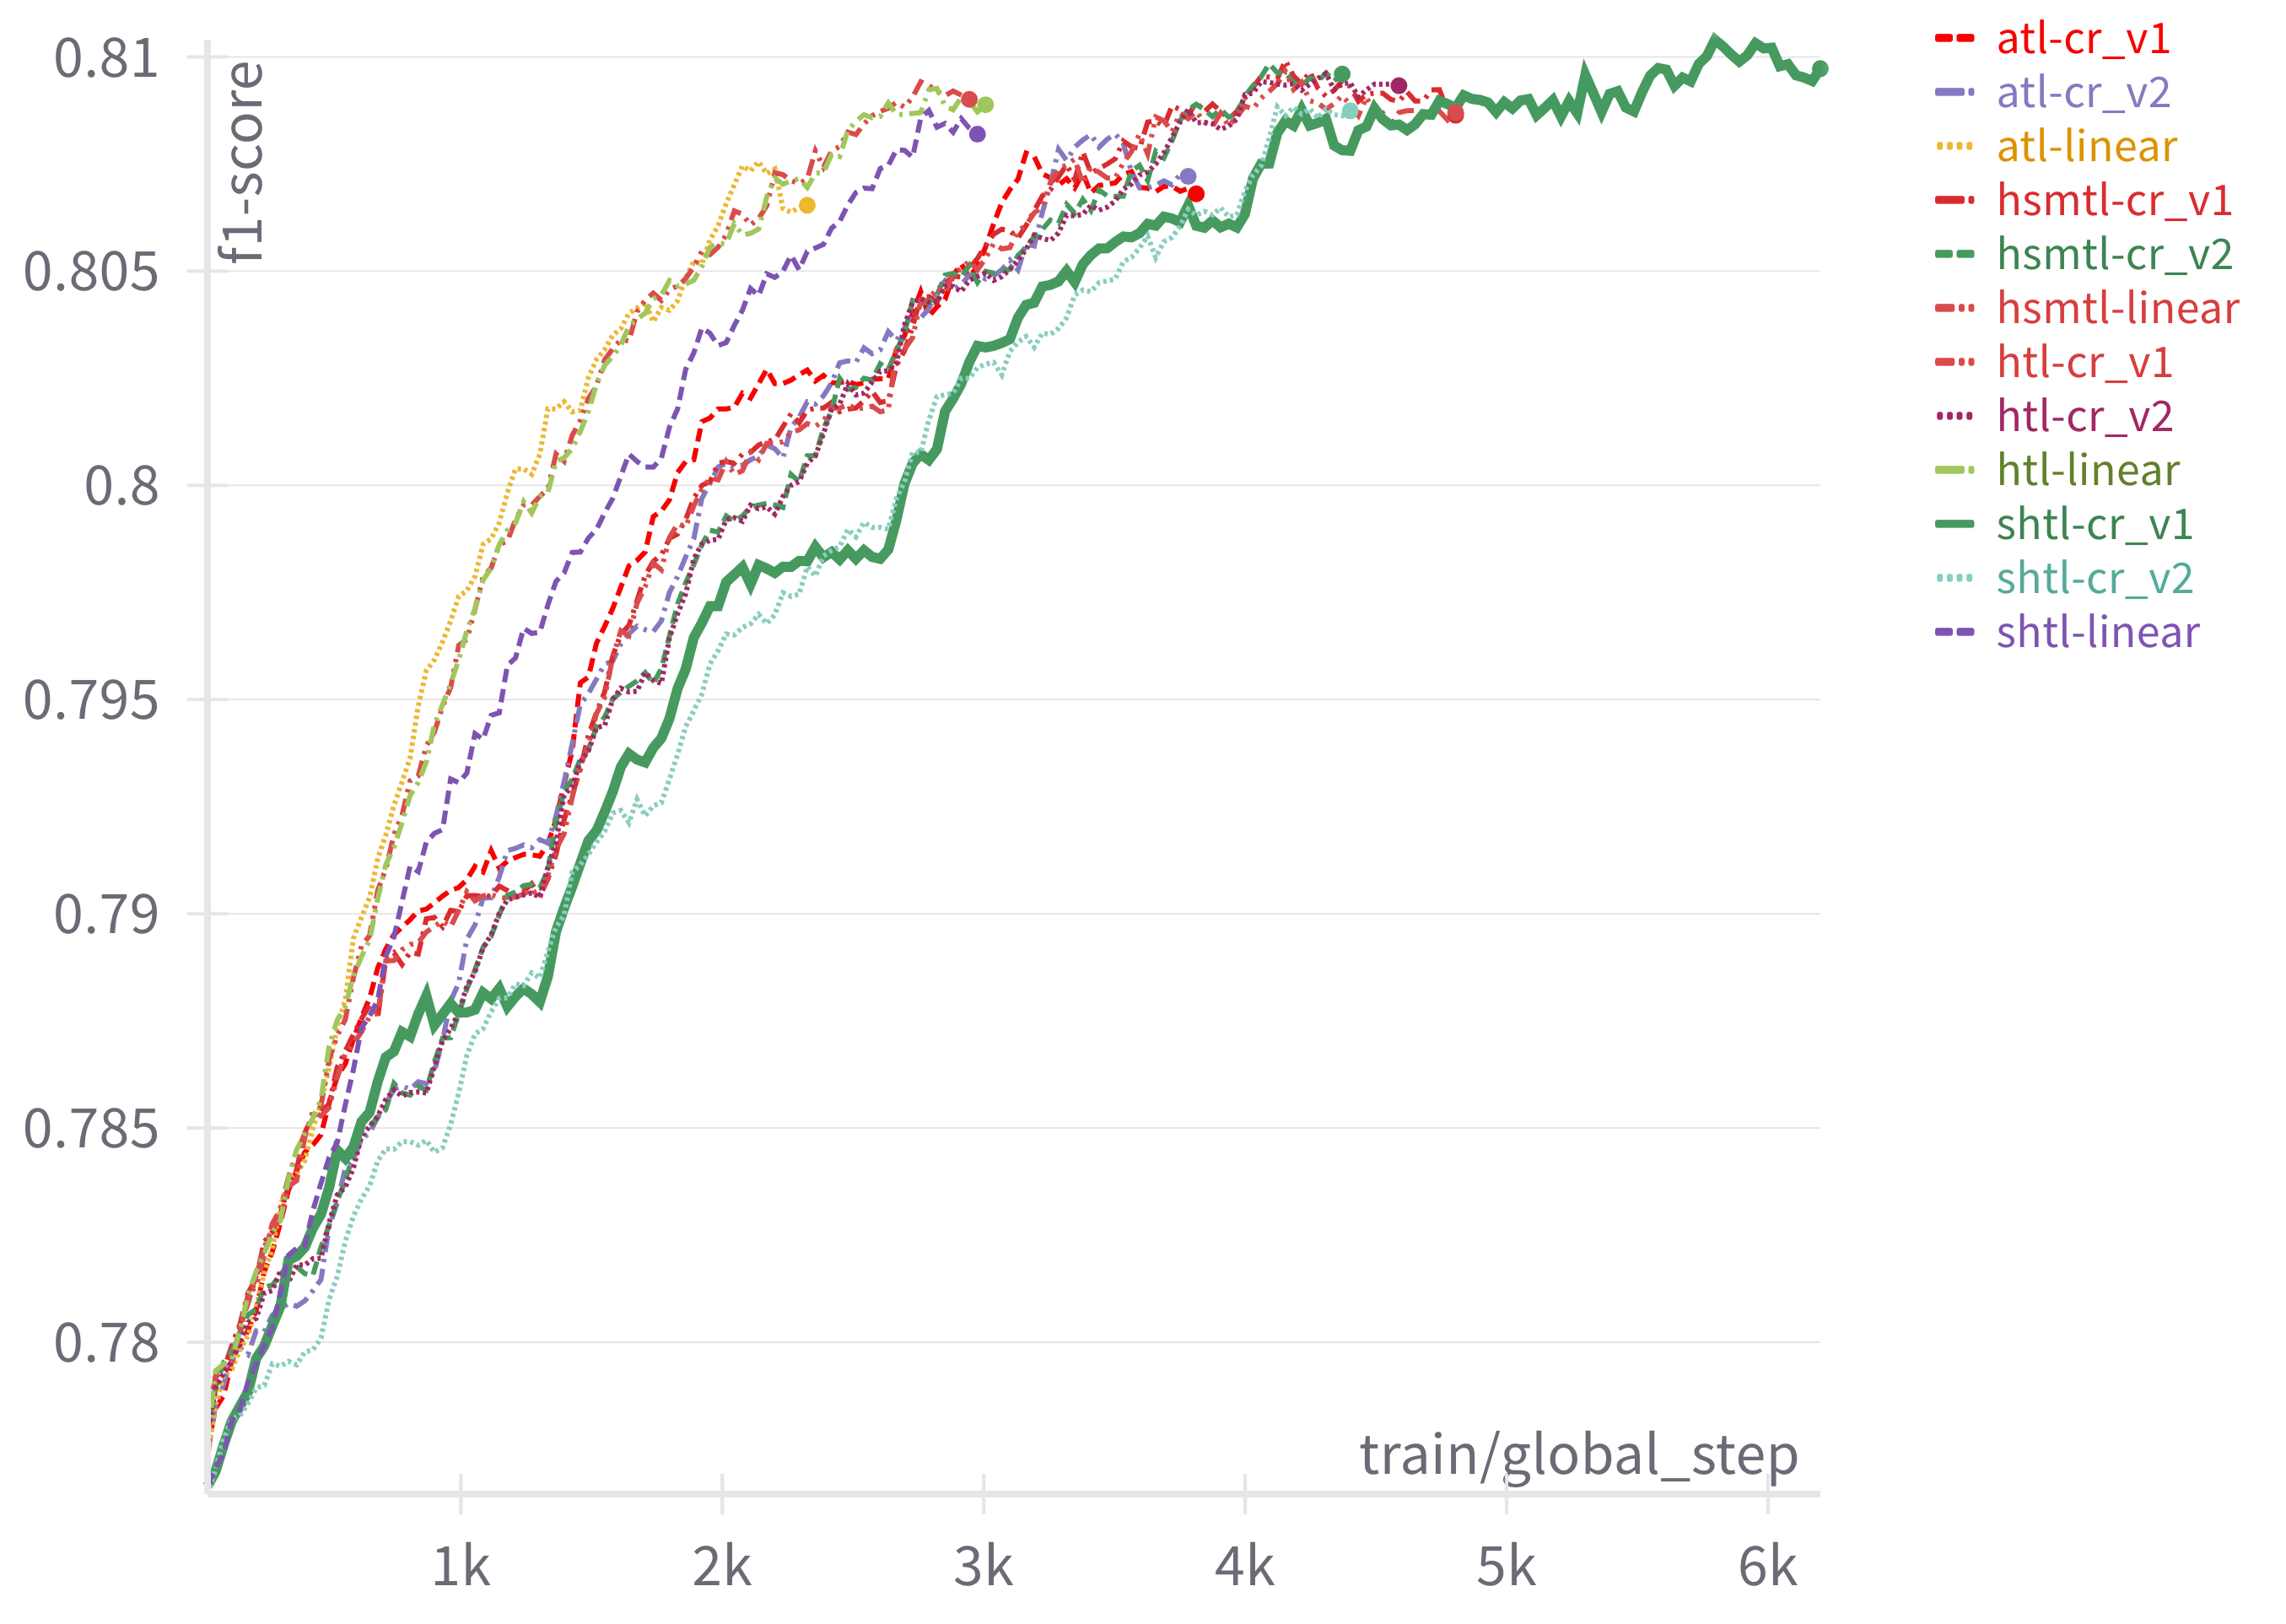
\includegraphics[scale=0.15,trim={0 0 0 0},clip]{Binary Classification Eval fine-tuning.png}
    \caption{Validation \(F_1\)-Score}
    % {\footnotesize Clockwise from bottom left: 4-class raw text, 3-class raw text, binary raw text, binary
    %     structured topics, 3-class structured topics, and 4-class structured topics.\\\footnotemark[1]ins: insufficient description}
    \label{fig:binaryf1}
\end{figure}

A visual inspection of the learning curves reveals several distinct patterns. The configurations utilizing \verb|BatchHardSoftMarginTripletLoss| seem to consistently demonstrate superior performance.  They exhibit some of the steepest learning curves, indicating faster convergence, and reach some of the highest peak \(F_1\)-scores, surpassing all loss function types.  The \verb|BatchHardTripletLoss| family of functions seem to perform similarly, albeit slightly worse. \verb|AllTripletLoss| configurations display the steepest learning curves, but show a performance collapse much earlier and at much lower \(F_1\)-score peaks than any of the other functions.  Finally, the \verb|BatchSemiHardTripletLoss| configurations exhibit the slowest learning curves, and do not seem to seem to reach the highest peak scores on average.  Nonetheless, it appears that its more erratic behavior near its plateau can produce results that surpass all other functions, possibly allowing it to leap out of a local minimum.  These visual trends strongly suggest that the choice of triplet mining strategy is a major factor in determining the training speed and final performance of the fine-tuned model for this task.

\subsubsection{Quantitative Performance Summary}
To provide a more precise and formal comparison, the exact peak validation \(F_1\)-scores achieved by each configuration are summarized in Table~\ref{tab:finetune_f1_scores}. This table distills the dynamic information from the learning curves into a single, quantitative metric for each experimental condition, enabling a direct and data-driven selection of the optimal configuration.
\begin{table}[tb]
    \captionsetup{skip=5pt}
    \centering
    \caption{Peak Validation F1-Score of Fine-Tuning Configurations on BGE Model}
    \label{tab:finetune_f1_scores}
    \resizebox{\columnwidth}{!}{
        \begin{tabular}{l c c c}
            \toprule
            \textbf{Loss Function}                          & \textbf{Linear Scheduler} & \textbf{Cosine Restarts v1} & \textbf{Cosine Restarts v2} \\
            \midrule
            \texttt{BatchAllTripletLoss} (atl)              & 0.8076                    & 0.8078                      & 0.8082                      \\
            \texttt{BatchHardSoftMarginTripletLoss} (hsmtl) & 0.8094                    & 0.8099                      & 0.8098                      \\
            \texttt{BatchHardTripletLoss} (htl)             & 0.8093                    & 0.8097                      & 0.8096                      \\
            \texttt{BatchSemiHardTripletLoss} (shtl)        & 0.8088                    & \textbf{0.8104}             & 0.8088                      \\
            \bottomrule
        \end{tabular}
    }
\end{table}
The quantitative data presented in the aforementioned table reveals a nuanced outcome that adds precision to the qualitative analysis of the learning curves. While the \verb|BatchHardTripletLoss| and \verb|BatchHardSoftMarginTripletLoss| configurations consistently achieved high scores across all schedulers, the single best-performing configuration was the combination of \verb|BatchSemiHardTripletLoss| and the \verb|cr_v1| learning rate schedule, which achieved the highest peak validation \(F_1\)-score of 0.8104. This result suggests that while aggressive hard-negative mining provides a strong and reliable performance floor, a more moderate semi-hard mining strategy, when paired with an appropriate cosine annealing schedule, can find a slightly better optimum for this specific task.

\subsection{Analysis and Selection of the Optimal Model}
The empirical results from the fine-tuning experiments point to a single optimal configuration. This section provides a detailed analysis of why this specific combination of components was most effective, grounding the observed performance in the theoretical principles of metric learning and optimization. The superiority of the chosen model is then validated through rigorous statistical testing.

\subsubsection{Identifying and Validating the Top Performer}
Based on the comprehensive results presented in Table~\ref{tbl:finetune_f1_scores}, the combination of \verb|BatchSemiHardTripletLoss| with the \verb|cr_v1| learning rate schedule, applied to the \verb|BAAI/bge-small-en-v1.5| base model, is the optimal configuration. The superior performance of this configuration arises from a delicate balance between a sufficiently challenging learning objective and a robust, adaptive optimization strategy.{\setlength{\emergencystretch}{5em}\par}

The course equivalency task is challenging because it demands the ability to make fine-grained semantic distinctions. The choice of triplet mining strategy is therefore critical. While a highly aggressive strategy like BatchHardTripletLoss provides a strong learning signal by focusing on the most confusing examples, it can also lead to training instability or convergence to sharp, suboptimal minima~\cite{hermans2017defensetripletlossperson,Schroff_2015_CVPR}. The winning strategy, \verb|BatchSemiHardTripletLoss|, offers a more balanced approach. It focuses on triplets where the negative sample is more distant than the positive but still violates the margin (\(d(a,p) < d(a,n) < d(a,p) + \mathrm{margin}\)). This ``semi-hard'' mining provides a useful, stable gradient for training by ignoring the easiest examples (which offer no learning signal) and the absolute hardest examples (which can introduce noise and instability)~\cite{Schroff_2015_CVPR}. For this dataset, this moderate approach proved most effective, allowing the model to steadily learn discriminative features without being derailed by extreme outliers, ultimately leading to a better final solution.{\setlength{\emergencystretch}{5em}\par}

This effective learning objective was paired with a sophisticated optimization strategy. The \verb|CosineAnnealingWarmRestarts| scheduler, first proposed by Loshchilov and Hutter, is designed for complex loss landscapes. Its periodic ``warm restarts,'' where the learning rate is abruptly reset, act as an escape mechanism, forcing the optimizer out of any local minimum it may have settled into and allowing it to explore other regions of the loss landscape~\cite{loshchilovhutter}. The \verb|cr_v1| schedule, with its 6 cycles and higher patience, provided a more measured exploration than the more aggressive v2 schedule. This slightly slower, more patient schedule likely gave the optimizer sufficient time to converge more deeply into a broad, high-quality minimum after each restart. The synergy between a stable learning signal (shtl) and a robust-yet-patient exploration strategy (\verb|cr_v1|) is likely what enabled the model to achieve the highest validation score.

The entire training process is underpinned by the AdamW optimizer. As established by Loshchilov and Hutter in their seminal work, AdamW's key innovation is the decoupling of weight decay from the gradient update step~\cite{loshchilov2019decoupledweightdecayregularization}. By applying weight decay directly to the weights after the gradient update, AdamW ensures a more stable and effective regularization, which is crucial for preventing the model from overfitting~\cite{loshchilov2019decoupledweightdecayregularization}. This synergistic framework, a balanced learner (shtl), a strategic explorer (CosineAnnealingWarmRestarts), and a stable foundation (AdamW), is what enabled the successful training of a highly discriminative model.

\subsubsection{Statistical Validation of the Fine-Tuned Model}
To definitively validate the overall benefit of the fine-tuning process, the performance of the fine-tuned model (bge-ft) was compared against the suite of off-the-shelf models. A preliminary comparison was conducted using the mean test scores from a comprehensive, brute force, cross-validation grid search.  Once the PPM data was acquired, the final final comparison was completed with a hold-out test set as described in Section~\ref{ch:3.2.1}.  This provides the most honest and unbiased assessment of the model's generalization capabilities.

The descriptive statistics reveal that bge-ft not only achieved the highest mean \(F_1\) test score (\(\mu = 0.9786\)) but also exhibited the lowest standard deviation (\(\sigma = 0.0045\)). This indicates that the fine-tuned model is not only more accurate on average but also more consistent in its performance on unseen data across different configurations of dimensionality reduction and classifiers.

To test for statistically significant differences, a one-way Analysis of Variance (ANOVA) was performed. The ANOVA test yielded a highly significant result (\(F=6.2856, p<0.001\)), rejecting the null hypothesis that all model groups have equal means. This confirms that there is a statistically significant difference in performance between at least two of the models on the test data.

Prior to post-hoc testing, the assumption of homogeneity of variances was checked using Levene's test (with the Brown-Forsythe correction). The test was significant (\(F=6.9305, p<0.001\)), indicating that the variances among the model groups were not equal. This violation of the homoscedasticity assumption makes standard post-hoc tests like Tukey's HSD inappropriate and correctly justifies the use of the Games-Howell post-hoc test, which does not assume equal variances.

The Games-Howell post-hoc test was used to conduct pairwise comparisons between all model groups. The fine-tuned bge-ft model demonstrated a statistically significant improvement over its base model, bge, with a mean \(F_1\)-score increase of 0.0109 (\(p<.001, 95\% CI [0.0054, 0.0164]\)). Notably, bge-ft significantly outperformed all other evaluated models, including those that were orders of magnitude larger. These differences were statistically significant, with bge-ft outperforming gist (\(p=0.0009\)), nve (\(p=0.0003\)), and sfr (\(p=.0115\)). One unexpected finding was that no statistically significant differences were found among the off-the-shelf models themselves. This provides strong evidence that the fine-tuning process led to a meaningfully superior and more reliable embedding model for this task.{\setlength{\emergencystretch}{5em}\par}

\subsection{The Final Fine-Tuned Model}
The objective of this fine-tuning process is not merely to improve classification accuracy but to leverage deep metric learning to engineer a bespoke embedding space. Deep metric learning seeks to learn a representation function that maps data samples into an embedding space where similarity can be measured directly as a distance. The goal is to produce embeddings where vectors for equivalent courses are clustered closely together, while vectors for non-equivalent courses are pushed far apart, thereby creating a more discriminative feature space for subsequent classification.

This rigorous evaluation leads to a clear and unambiguous conclusion. The single best model for this task is the \verb|BAAI/bge-small-en-v1.5| model fine-tuned using \verb|BatchSemiHardTripletLoss| and a \verb|CosineAnnealingWarmRestarts| learning rate schedule (\verb|cr_v1|). This model, designated as bge-ft, not only demonstrated the highest performance during validation but was also proven to be statistically superior to all off-the-shelf models evaluated in this study, including its own foundation model. Therefore, this bge-ft model will be carried forward as the primary fine-tuned embedding model for the comprehensive classifier evaluation detailed in the next section.{\setlength{\emergencystretch}{5em}\par}

\section{Classifier Evaluation}
This section presents the definitive, multi-stage evaluation of the downstream classifiers, which represents the final component of the proposed framework. The primary objective is to systematically identify the optimal classification model for the course equivalency task, balancing the dual requirements of predictive accuracy and computational efficiency. The evaluation process is designed as a funnel, beginning with a broad preliminary review of eight distinct models on an initial dataset to identify the most promising algorithmic families. This is followed by a more focused and rigorous analysis of four finalist classifiers on the larger, more comprehensive PPM Corpus. This final stage includes an examination of the trade-off between model efficacy and efficiency, culminating in a statistically robust comparison on held-out test data to determine the single best-performing model for this application.

% \subsection{Introduction to Classifier Evaluation}
% The goal of this evaluation is to systematically identify the optimal downstream classifier for the course equivalency task. This is achieved through a multi-stage evaluation process designed to balance classification performance with practical deployment considerations, such as computational cost. The process begins with a broad preliminary review on the Initial Dataset to identify top-performing models and algorithmic families, efficiently narrowing the field of candidates. This is followed by a detailed, in-depth analysis of the selected finalists using the larger and more robust PPM Corpus. This second stage focuses on assessing the trade-off between efficacy (accuracy) and efficiency (computational cost) and concludes with a formal statistical analysis to identify the single best model. This section serves as the culmination of the entire pipeline, where the quality of the engineered features and fine-tuned embeddings is ultimately tested by their ability to drive accurate and efficient classification.

\subsection{Preliminary Classifier Performance Review (Initial Dataset)}
The first stage of the evaluation was a wide-ranging initial assessment of eight different machine learning models, conducted to identify the most effective algorithmic families and select the strongest candidates for the final, in-depth analysis. This preliminary review was conducted using the Initial Dataset, a manually curated corpus of 5,660 equivalent and 5,660 non-equivalent course pairs derived from established articulation agreements.

The evaluation tested a diverse suite of eight classifiers: Logistic Regression (LR), Ridge, Lasso, K-Nearest Neighbors (KNN), Support Vector Machine (SVM), Random Forest (RF), Linear Discriminant Analysis (LDA), and Quadratic Discriminant Analysis (QDA). These models were tested against multiple feature sets derived from the three primary off-the-shelf embedding models (BGE, GIST, NVE). The feature sets were further varied by applying multiple dimensionality reduction techniques (PCA, t-SNE, PaCMAP) and, critically, by testing configurations with and without the engineered cosine similarity feature. The evaluation was performed using a brute-force hyperparameter grid search with 5-fold cross-validation, with the \(F_1\)-score as the primary performance metric. The comprehensive results of this preliminary evaluation are presented in Table 4.5.

\subsubsection{Analysis of Linear Classifiers (LR, Ridge, Lasso, LDA)}
The linear models, which served as a performance baseline, revealed a profound dependency on the engineered global similarity feature. As shown in Table 4.5, their performance was consistently mediocre when trained only on the element-wise difference vector, but improved dramatically with the inclusion of the single cosine similarity term. For instance, using the BGE embeddings with no dimensionality reduction, the \(F_1\)-score for Logistic Regression surged from 0.6859 to 0.9013. Similar gains were observed for Ridge (0.6901 to 0.9066), Lasso (0.6826 to 0.9093), and LDA (0.6876 to 0.9068).

This behavior highlights the inherent limitations of linear models for this task. These models can only learn linear decision boundaries. The high-dimensional element-wise difference vector, by itself, represents a complex, non-linear relationship between courses that these models are incapable of capturing. The single, engineered cosine similarity feature provides a highly informative, globally relevant, and, most importantly, linearly separable signal. It acts as a ``shortcut,'' effectively pre-processing the complex relationship into a simple feature that the linear model can easily exploit. The element-wise difference vector contains granular, local information, while the cosine similarity contains holistic, global information. Linear models are poor at aggregating this local information into a global understanding but are excellent at exploiting a pre-computed global feature. This finding strongly validates the design of the composite distance vector, \(\Delta_c\).

\subsubsection{Analysis of Non-Linear Classifiers (KNN, SVM, RF, QDA)}
In stark contrast, the group of non-linear models significantly and consistently outperformed their linear counterparts. Critically, their performance was largely insensitive to the inclusion or omission of the cosine similarity feature. As seen in Table 4.5, using the BGE embeddings with no dimension reduction, the SVM classifier achieved near-perfect \(F_1\)-scores of 0.9988 without the cosine feature and 0.9983 with it. Likewise, KNN scored 0.9818 versus 0.9833, and Random Forest scored 0.9830 versus 0.9807. The differences are negligible, indicating that the engineered global feature was redundant for these models.

This indifference suggests that these more complex models possess sufficient capacity to implicitly reconstruct the global relationship directly from the high-dimensional local difference vector. An SVM with a non-linear kernel, a Random Forest aggregating many decision trees, or a KNN model operating on local neighborhood density can all create highly complex decision surfaces. These mechanisms are powerful enough to infer that a small magnitude in the difference vector across many dimensions equates to high global similarity. They do not need the explicit ``shortcut'' that the linear models rely on; they can deduce the global relationship from the local information provided, rendering the explicit cosine feature unnecessary.

\subsubsection{Impact of Dimensionality Reduction and Anomalous Results}
For the top-performing non-linear models (KNN, SVM, RF), dimensionality reduction generally had a neutral or slightly negative impact on performance. For example, with BGE embeddings and the cosine feature, SVM's \(F_1\)-score dropped from 0.9983 (no reduction) to 0.9772 (4D PCA), suggesting that the reduction techniques, while reducing complexity, also discarded some useful, discriminative information from the high-dimensional embeddings.

A notable exception was the highly erratic behavior of QDA. Without dimensionality reduction, its performance was abysmal, with an \(F_1\)-score as low as 0.0410 for BGE embeddings. However, with dimensionality reduction, its performance became competitive (e.g., 0.9518 for 4D PCA). 1  This is a classic symptom of QDA's statistical assumptions being violated in high-dimensional space. QDA assumes that each class has its own covariance matrix and that these matrices are invertible. When the number of features (e.g., 384 for BGE) is much larger than the number of samples per class, the sample covariance matrices can become ill-conditioned or singular (not invertible), leading to numerical instability and catastrophic failure. Dimensionality reduction projects the data into a lower-dimensional space, creating a more stable, well-behaved covariance matrix that QDA can handle, thus ``rescuing'' its performance. This instability makes QDA an unreliable and unsuitable candidate for this task.

\subsubsection{Selection of Finalists}
The preliminary results clearly identified K-Nearest Neighbors (KNN), Support Vector Machine (SVM), and Random Forest (RF) as the most successful and robust classifiers. These three models consistently delivered the highest \(F_1\)-scores, with results ranging from 0.916 to 0.999 across various configurations. To complete the final slate for the more rigorous evaluation, XGBoost (XGB) was added. This was done to include a state-of-the-art gradient boosting implementation, known for its high performance on structured data, ensuring the final comparison included a top-tier boosting algorithm alongside instance-based, kernel, and bagging ensemble methods. These four models, KNN, SVM, RF, and XGB, were carried forward for the final, definitive evaluation on the PPM Corpus.

\subsection{Efficacy vs. Efficiency}
This subsection transitions the analysis from the Initial Dataset to the larger, more robust PPM Corpus. The focus now shifts to investigating the crucial trade-off between model performance (efficacy) and computational cost (efficiency) for the four finalist classifiers. The analysis is based on aggregated data from the extensive cross-validation grid search performed during model training on this new corpus. Figure~\ref{fig:f1time} visualizes this trade-off by plotting the median of mean \(F_1\)-scores from the hyperparameter grid search against both training and inference times for each classifier configuration tested.
\begin{figure}[tb]
    \captionsetup{skip=5pt}
    \centering
    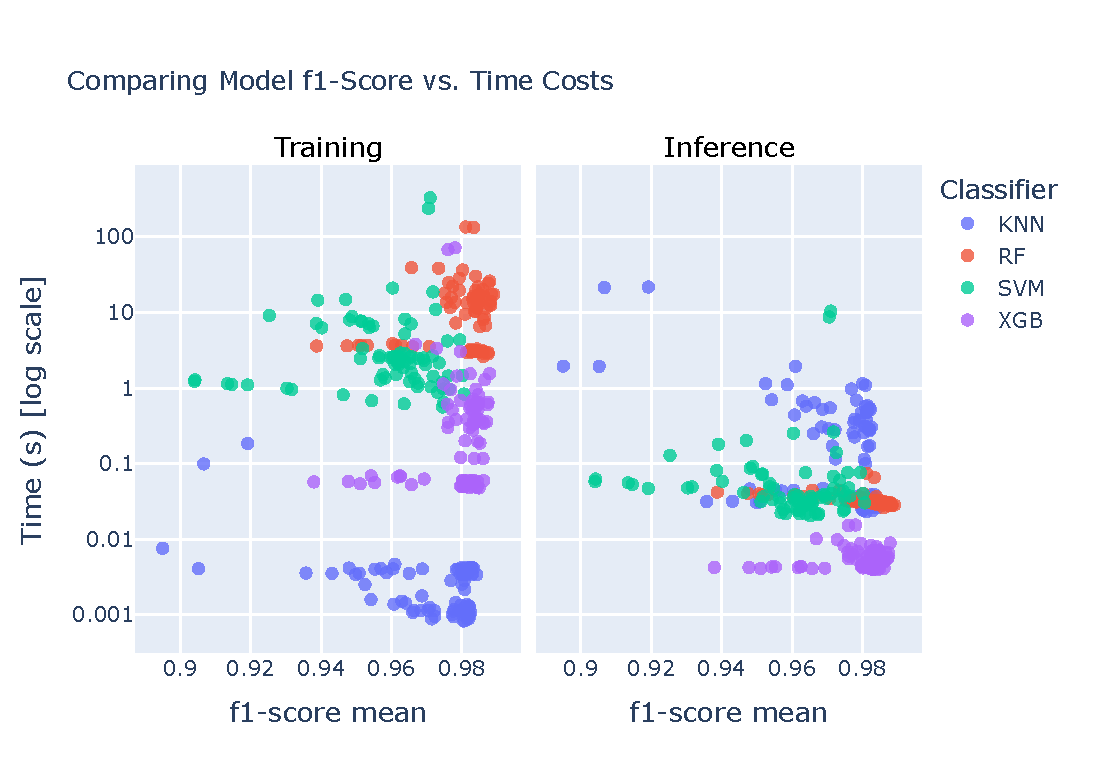
\includegraphics[scale=0.85,trim={0 5mm 0 18mm},clip]{cv_f1 vs time.pdf}
    \caption{Classifier \(F_1\)-Score vs. Training and Inference Time}
    % {\footnotesize Clockwise from bottom left: 4-class raw text, 3-class raw text, binary raw text, binary
    %     structured topics, 3-class structured topics, and 4-class structured topics.\\\footnotemark[1]ins: insufficient description}
    \label{fig:f1time}
\end{figure}

\subsubsection{Training Time vs. \(F_1\)-Score}
The left panel of Figure~\ref{fig:f1time} shows a wide distribution of long training times required to achieve high \(F_1\)-score means, particularly for the RF and SVM classifiers. Some configurations for these models require over 10 seconds to train, while others are much faster. KNN and XGBoost, in contrast, are more consistently located in the lower range of training times, often under 1 second. This indicates that while high-performing models do not necessarily require the longest training times, an exhaustive search to find the optimal configuration can be computationally expensive.

\subsubsection{Inference Time vs. \(F_1\)-Score}
The right panel of Figure~\ref{fig:f1time} reveals the most critical efficiency metric for a practical, scalable production system: inference time. Here, Random Forest and XGBoost emerge as the clear winners. Their data points are tightly clustered in the bottom-right of the high-\(F_1\)-score region, with inference times consistently under 0.1 seconds. In contrast, SVM and KNN, while capable of high performance, show much greater variability and significantly slower inference times in many configurations. Some high-performing KNN and SVM models have inference times approaching or exceeding 0.1 seconds—an order of magnitude slower than Random Forest and XGBoost.

This finding has significant practical implications. Inference time, not training time, directly impacts the latency and responsiveness of a deployed system. The wide plume of inference times for KNN and SVM represents an operational risk; while a fast configuration could be selected, a model retrained on new data might inadvertently select a ``slow'' set of hyperparameters, degrading system performance. The tight clustering for Random Forest and XGBoost indicates that their efficiency is a stable and predictable property. This reliability makes them inherently more robust choices for deployment in a real-world, low-latency application where consistent performance is paramount.

While all four finalists can achieve excellent accuracy on the PPM corpus, Random Forest and XGBoost offer a more consistently efficient path to high performance, making them strong candidates for a production environment.

\subsection{Statistical Analysis of Classifier Performance}
The objective of this final stage is to conduct a definitive and statistically rigorous comparison of the four finalist classifiers using the held-out test data from the PPM Corpus. This analysis moves beyond descriptive summaries to formal hypothesis testing to declare a statistical winner based on generalization performance on unseen data.

\subsubsection{Distribution of \(F_1\)-Scores}
As shown in Table~\ref{tbl:clsdescstat} and Figure~\ref{fig:clscoredist}, all four classifiers demonstrate exceptionally high and stable performance on the test data. The mean \(F_1\)-scores are clustered in a very tight range, from 0.970 (RF) to 0.976 (SVM). Notably, the Support Vector Machine (SVM) model achieved the highest mean \(F_1\)-score (\(\mu = 0.975973\)). Furthermore, it also exhibited the lowest standard deviation (\(\sigma = 0.009120\)). This combination of the highest mean and lowest variance indicates that SVM is not only the most accurate classifier on average but also the most consistent and reliable performer across the various feature sets.
\begin{figure}[tb]
    \captionsetup{skip=5pt}
    \centering
    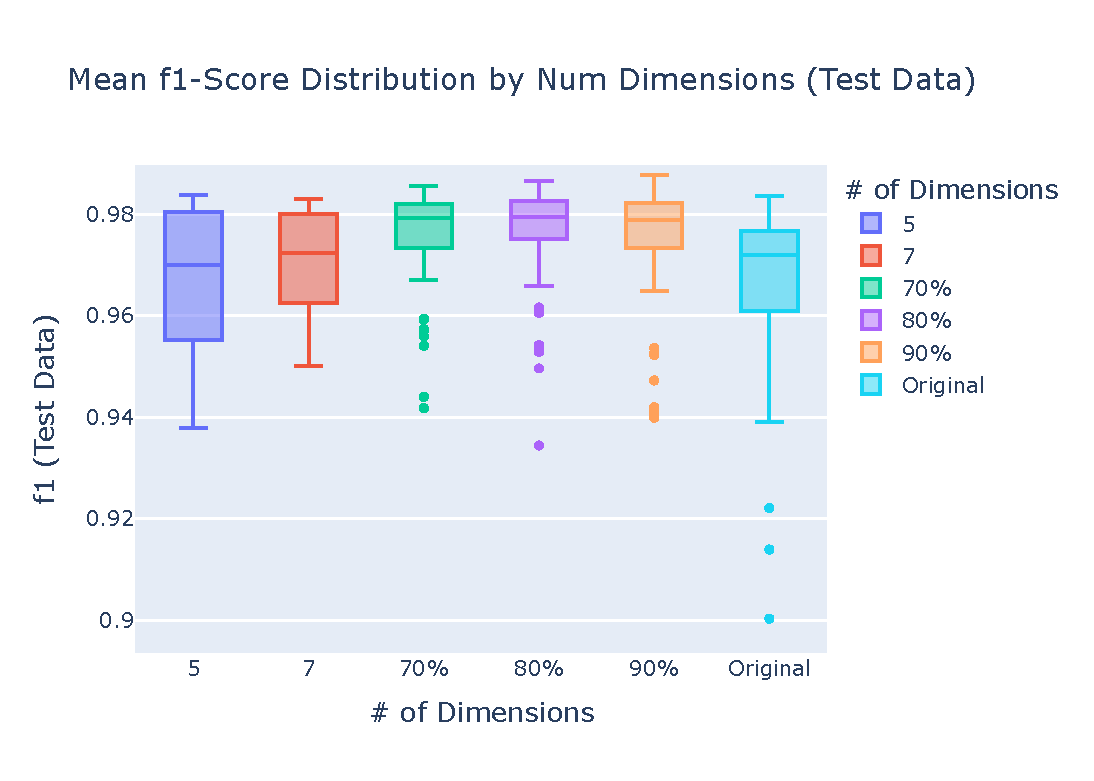
\includegraphics[scale=0.75,trim={0 5mm 0 18mm},clip]{classifier_f1score_boxplot_test.pdf}
    \caption{\(F_1\)-Score Distribution of Finalist Classifiers}
    % {\footnotesize Clockwise from bottom left: 4-class raw text, 3-class raw text, binary raw text, binary
    %     structured topics, 3-class structured topics, and 4-class structured topics.\\\footnotemark[1]ins: insufficient description}
    \label{fig:clscoredist}
\end{figure}
\begin{table}[tb]
    \captionsetup{skip=5pt}
    \caption{Model Specifications and Performance}
    \label{tbl:clsdescstat}
    \centering
    \resizebox{\columnwidth}{!}{
        \begin{tabular}{lcccccccc}
            \toprule                                                                                        \\
            Classifier & Count & Mean     & Std      & Min      & 25\%     & 50\%     & 75\%     & Max      \\
            \midrule
            KNN        & 80.0  & 0.971147 & 0.015208 & 0.900304 & 0.971809 & 0.977110 & 0.979110 & 0.982437 \\
            RF         & 80.0  & 0.970397 & 0.014636 & 0.934443 & 0.957361 & 0.978490 & 0.982108 & 0.984572 \\
            SVM        & 80.0  & 0.975973 & 0.009120 & 0.939885 & 0.970523 & 0.979408 & 0.982786 & 0.987702 \\
            XGB        & 80.0  & 0.971026 & 0.012316 & 0.942860 & 0.959382 & 0.977547 & 0.981376 & 0.984898 \\
            \bottomrule
        \end{tabular}
    }
\end{table}

\subsubsection{Statistical Validation of Classifiers}
To determine if the observed differences in mean performance were statistically significant, a formal hypothesis testing procedure was conducted. The results are summarized in Table~\ref{tab:cls_agh}.
\begin{table}[tb]
    \captionsetup{skip=5pt}
    \centering
    \caption{Summary of ANOVA and Games-Howell Post-Hoc Test Results}
    \label{tab:cls_agh}
    \begin{tabular}{l}
        \toprule
        \textbf{Test}                                                                                                      \\
        \midrule
        \textbf{One-way ANOVA}                                                                                             \\
        \quad \(H_0: \mu_{\textrm{KNN}} = \mu_{\textrm{RF}} = \mu_{\textrm{SVM}} = \mu_{\textrm{XGB}}\) (All classifier means are equal)                         \\
        \quad \(H_a\): At least one classifier mean is different                                                             \\
        \quad \(F(3, 316) = 3.1293, p = 0.02596\)                                                                            \\
        \quad \textit{Result: Reject \(H_0\). Significant difference between groups.}                                        \\
        \midrule
        \textbf{Levene's Test (Brown-Forsythe)}                                                                            \\
        \quad \(H_0: \sigma^2_{\textrm{KNN}} = \sigma^2_{\textrm{RF}} = \sigma^2_{\textrm{SVM}} = \sigma^2_{\textrm{XGB}}\) (All classifier variances are equal) \\
        \quad \(H_a:\) At least one classifier variance is different                                                         \\
        \quad \(F = 2.7883, p = 0.0408\)                                                                                     \\
        \quad \textit{Result: Reject \(H_0\). Variances are unequal.}                                                        \\
        \toprule
        \textbf{Games-Howell Post-hoc Test}                                                                                \\
        \begin{tabular}{l l r r r}
            \toprule
            \textbf{group1} & \textbf{group2} & \textbf{meandiff} & \textbf{p-adj} & \textbf{reject} \\
            \midrule
            KNN             & RF              & -0.0008           & 0.9888         & False           \\
            KNN             & SVM             & 0.0048            & 0.0757         & False           \\
            KNN             & XGB             & -0.0001           & 0.9999         & False           \\
            RF              & SVM             & 0.0056            & 0.0229         & \textbf{True}   \\
            RF              & XGB             & 0.0006            & 0.9911         & False           \\
            SVM             & XGB             & -0.0049           & 0.0229         & \textbf{True}   \\
        \end{tabular}\\
        \bottomrule
        \multicolumn{1}{p{14cm}}{This table summarizes the results of the inferential tests on the classifier \(F_{1}\)-scores from the held-out test data.}
    \end{tabular}
\end{table}
A one-way Analysis of Variance (ANOVA) was first performed to test the null hypothesis that all four classifiers have equal mean \(F_1\)-scores. The test yielded a statistically significant result (\(F(3,316)=3.1293,p=0.02596\)), allowing for the rejection of the null hypothesis and confirming that a significant difference exists among the classifiers.  

This result justified a post-hoc analysis to identify which specific pairs of classifiers differ. Prior to this, the assumption of homogeneity of variances was checked using Levene's Test (with the Brown-Forsythe correction). The test was significant (\(p=0.0408\)), indicating that the group variances were unequal. This violation correctly justifies the use of the Games-Howell post-hoc test, which does not assume equal variances, demonstrating methodological rigor.  

The Games-Howell test revealed that the SVM classifier performed statistically significantly better than both Random Forest (mean difference \(= 0.0056, p=0.0229\)) and XGBoost (mean difference \(= 0.0049, p=0.0229\)). No other pairwise differences were found to be statistically significant.  

While all four classifiers are unequivocally top-tier performers on the PPM test data, the formal statistical analysis identifies SVM as the definitive winner. It demonstrates a small but statistically significant advantage in accuracy and precision over both RF and XGBoost, solidifying its position as the most accurate model.

\subsection{Final Classifier Selection}
This multi-stage evaluation reveals a classic trade-off between peak performance and operational efficiency. The preliminary analysis on the Initial Dataset established the clear superiority of non-linear models (KNN, SVM, RF) over their linear counterparts, validating the need for classifiers that can handle the complexity of the high-dimensional feature vectors. The subsequent, more rigorous analysis on the PPM Corpus named SVM as the most accurate and precise model. However, the efficiency analysis highlighted that SVM can be computationally more expensive, particularly in terms of inference time, than the highly efficient Random Forest and XGBoost models.

The final choice is not a simple declaration of a single ``best'' model but a nuanced decision based on the specific deployment context. This represents a classic engineering dilemma: optimizing for peak performance versus optimizing for operational efficiency and scalability. The statistical significance of SVM's superiority, while real, results in a mean \(F_1\)-score improvement of approximately 0.5\%. For a batch-processing task where results are computed periodically and maximum accuracy is the only goal, this marginal gain might be worth the extra computational cost. However, for a real-time, interactive system serving many queries, the order-of-magnitude speed improvement and predictable low latency of Random Forest or XGBoost may be far more valuable than the small accuracy bump.

Based on the comprehensive evidence, the following final recommendations are made:
\begin{itemize}
    \item For Maximum Accuracy: The Support Vector Machine (SVM) is the recommended classifier for any scenario where achieving the absolute highest accuracy and consistency is the paramount objective. Its statistically significant advantage on the held-out test data makes it the definitive choice for performance-critical applications.
    \item For Optimal Efficiency: For applications where inference speed, low latency, and predictable performance are critical for scalability (e.g., real-time interactive systems), Random Forest and XGBoost represent highly compelling and practical alternatives. They provide nearly equivalent accuracy but with demonstrably superior and more reliable computational efficiency.
\end{itemize}

\section{Misclassification Analysis}
While the quantitative evaluation presented in Section 4.5 establishes the superior performance of the fine-tuned BGE model (bge-ft) based on aggregate metrics like the \(F_1\)-score, a purely numerical analysis is insufficient for a complete understanding of the system's behavior. High-level metrics are essential for benchmarking and model selection, but they obscure the underlying nature of a model's failures. They quantify what the performance is but fail to explain why and how errors occur. Relying on such metrics alone can be misleading, as they may overestimate a model's robustness while hiding significant, systematic failure modes~\cite{gauthier2022}. A critical step in the development of reliable and trustworthy AI systems is a thorough and systematic error analysis that moves beyond aggregate scores to diagnose specific weaknesses.

This section transitions from quantitative assessment to qualitative diagnosis. The objective is to perform a systematic error analysis on the misclassifications produced by the embedding models to understand the root causes of their failures. This investigation follows a two-pronged methodology. First, it examines systematic error patterns by analyzing the overlap of misclassified course pairs between different embedding models. This approach helps distinguish between model-specific weaknesses and challenges that are inherent to the dataset itself. Second, it conducts a granular, qualitative analysis of specific false positive and false negative examples drawn from the held-out test and cross-validation reports. This manual, case-based review is a cornerstone of effective error analysis, enabling the identification of specific artifacts and conceptual flaws that quantitative metrics cannot reveal. The overarching goal is to generate a structured report of the primary error types to inform future improvements to the system.

\subsection{Shared Misclassifications Across Models}
To diagnose the source of model errors, it is first necessary to determine whether they are idiosyncratic to individual models or systematic across them. If misclassifications are largely unique to each model, the errors are likely attributable to model-specific factors, such as architectural differences or suboptimal fine-tuning. Conversely, a significant overlap in misclassified pairs across multiple, diverse models would suggest the presence of systematic errors, failures that stem not from the models but from the data itself. Such errors often arise from annotation artifacts, inherent ambiguity in the source text, or insufficient information to support a clear classification, and they represent a fundamental challenge for any model applied to the dataset.

An analysis of the misclassifications on the held-out test data reveals a high degree of overlap, providing strong evidence for the prevalence of systematic errors. Figure~\ref{fig:venn_misclassified} presents a Venn diagram illustrating the intersection of misclassified pairs among the five evaluated embedding models. The most telling feature of this diagram is the central region, which shows that 211 distinct course pairs were misclassified by every single model, from the large, general-purpose gist and sfr models to the small, domain-specific bge-ft. This substantial number of universally challenging pairs immediately points to characteristics within the data that consistently confound semantic analysis.
\begin{figure}[tb]
\centering
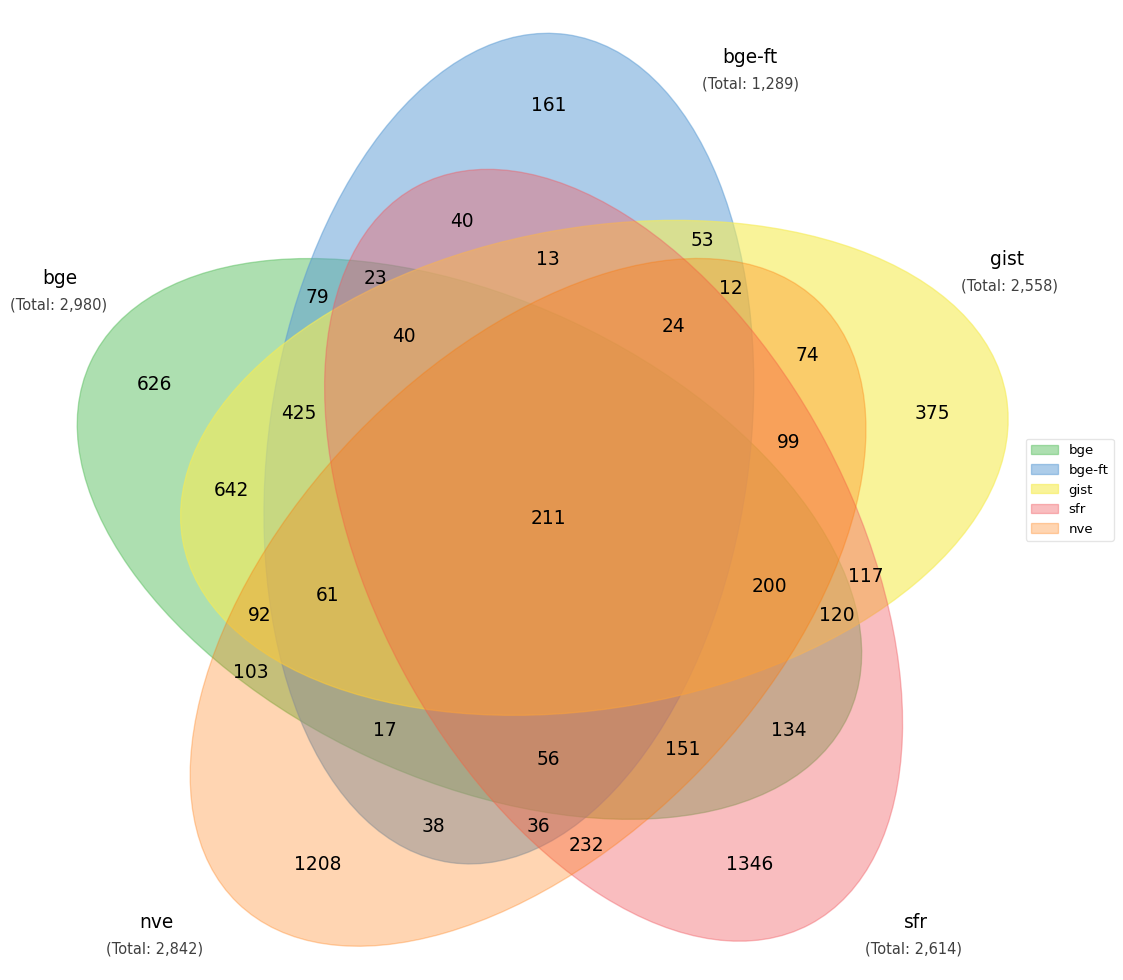
\includegraphics[width=0.8\textwidth]{venn_with_totals_evaldata.png}
\caption{Venn diagram illustrating the overlap of misclassified pairs on the test dataset between all five embedding models. The central intersection shows 211 pairs were misclassified by all models, indicating systematic data challenges.}
\label{fig:venn_misclassified}
\end{figure}

A more granular view, provided by the intersection bar charts in Figure~\ref{fig:intersection_barchart}, reinforces this finding. The chart shows the total number of misclassifications common to every possible combination of models. For example, the off-the-shelf bge and gist models share 1791 misclassified pairs. Even the top-performing fine-tuned model, bge-ft, shares 839 of its errors with gist and 912 with the base bge model. The fact that fine-tuning on domain-specific data, while improving the overall score, could not resolve these shared errors indicates that they are particularly resilient and likely stem from deep-seated issues within the source descriptions.
\begin{figure}[tb]
\centering
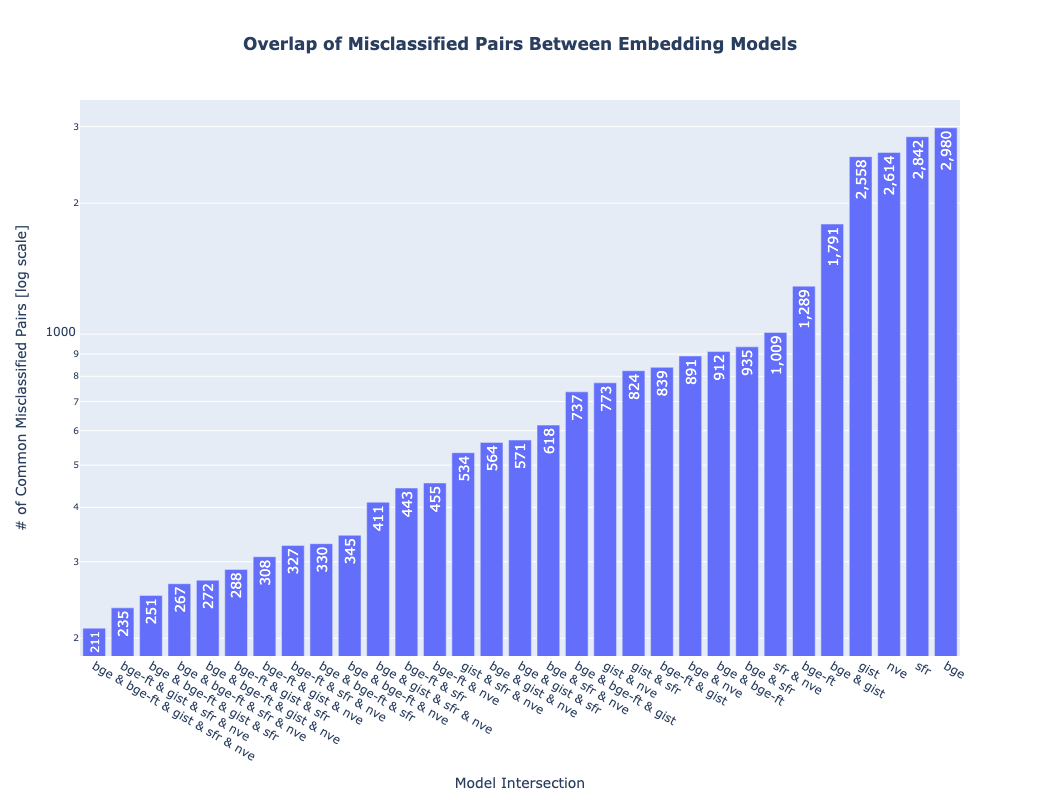
\includegraphics[width=\textwidth,trim={0 5mm 0 18mm},clip]{intersection_barchart_evaldata.png}
\caption{Number of common misclassified pairs between all model combinations on the test dataset. The high counts of shared errors across different models point to systematic challenges inherent in the data.}
\label{fig:intersection_barchart}
\end{figure}

The interpretation of this evidence is clear: a significant portion of the model failures are not random but are systematic products of the course catalog corpus. These ``hard'' examples consistently challenge a range of semantic embedding models, regardless of their pre-training data, architecture, or fine-tuning strategy.  It is possible that course equivalency may not even be possible with these challenging examples simply due to insufficient information or ambiguous phrasing. These systematic errors may define the performance ceiling of a purely course description approach and strongly suggest that further, more significant improvements will require methodologies that directly address the quality and nature of the data itself.

\subsection{Qualitative Analysis of False Positives}
A False Positive (FP) in this classification context occurs when the system incorrectly classifies two distinct, non-equivalent courses as being equivalent. This type of error carries significant real-world consequences. In an academic advising application, an FP could lead to a student being incorrectly advised that a course they plan to take will satisfy a transfer requirement, when in fact it will not. This could result in the student wasting time, effort, and tuition on a non-transferable course, potentially delaying their graduation. The following analysis, based on examples from the cross-validation and test reports, categorizes the primary causes of these harmful errors.

\subsubsection{Topical Overlap without True Equivalence}
This error category arises when two courses cover the same broad subject matter but differ in critical dimensions such as academic level, scope, depth, or their position within a curriculum sequence. The model correctly identifies the high semantic similarity based on shared keywords and concepts but fails to capture the nuanced distinctions that make the courses non-equivalent from a curricular standpoint. This reflects a core challenge in Semantic Textual Similarity (STS), which is distinguishing true meaning equivalence from mere topical relatedness.

A clear example of this is the false positive pair (1705, 1710) gathered from the cross-validation data. This pair consists of two courses from Foothill College: PHYS-4D General Physics (Calculus) and PHYS-4A General Physics (Calculus).
\begin{itemize}
    \item PHYS-4D Description: ``Special relativity, statistical mechanics, quantum mechanics, atomic physics, nuclear physics, particle physics\dots''
    \item PHYS-4A Description: ``Mathematics-physics interrelationships, classical Newtonian mechanics\dots''
\end{itemize}
Both courses are titled ``General Physics (Calculus)'' and share a similar structure, creating a high degree of semantic overlap that the model correctly detects. However, their ground-truth C-IDs (PHYS-215 for 4D and PHYS-200 for 4A) and their topic lists clearly indicate they are distinct courses in a multi-semester sequence. PHYS-4A covers foundational classical mechanics, while PHYS-4D covers advanced modern physics. The model's failure lies in its inability to discern this sequential, non-equivalent relationship, a crucial nuance for course articulation that is not fully encoded in the raw semantic content.

\subsubsection{Ambiguous or Vague Course Descriptions}
This error type occurs when course descriptions are too brief or use generic, high-level language, lacking the specific keywords and detailed concepts needed to differentiate them from other courses. This is a known challenge in the field of short-text semantic similarity, where a lack of rich context and descriptive detail inherently increases ambiguity and the likelihood of spurious matches~\cite{app13063911}.

A course prone to this type of error is COMM-1 Communication Fundamentals from Saddleback College. Its description is highly abstract:
\begin{itemize}
    \item COMM-1 Description: ``Understand and use the processes of communication in making personal and social decisions in everyday life, including an understanding of problems and propositions; organization and development of ideas; evidence; methods of research, criticism and evaluation. Presentation of ideas in informative and persuasive contexts\dots''
\end{itemize}

The language used---``processes of communication,'' ``development of ideas,'' ``presentation of ideas''---is so general that it could be semantically close to a wide range of courses, including public speaking, critical thinking, rhetoric, or even introductory philosophy. This lack of specificity provides a weak and ambiguous signal to the embedding model, making it highly susceptible to generating false positives when compared with other generically described introductory courses.

\subsection{Qualitative Analysis of False Negatives}
A False Negative (FN) occurs when the system fails to identify an equivalence between two courses that are, according to the ground truth, officially equivalent. In a practical application, this error represents a missed opportunity for a student. It could lead to a student being incorrectly advised that they need to retake a course for which they should have received credit, hindering their academic progress and incurring unnecessary costs. The analysis of FN examples reveals that these errors are predominantly a consequence of inconsistencies and information gaps in the source data.

\subsubsection{Semantic Divergence in Descriptions}
This error occurs when two officially equivalent courses are described using vastly different terminology, phrasing, or thematic focus. While the courses satisfy the same curricular requirement, their textual descriptions are semantically distant. This is a classic challenge in domain-specific NLP, where institutional ``dialects,'' varying authoring styles, or different pedagogical emphases can obscure an underlying equivalence that is not apparent from the text alone.

The false negative pair (516, 752) from the test data, both with the C-ID CDEV-100, is a powerful illustration of this phenomenon.
\begin{itemize}
    \item Foothill College, CHLD-2 Description: ``Development of the child from middle childhood through adolescence. This introductory course examines the major physical, psychosocial, and cognitive/language developmental milestones for children\dots''
    \item Cerritos College, CD-110 Description: ``Examines the historical and current perspectives on diversity and inclusion and the impact of systemic societal influences on children's development, learning, and school experiences. Strategies for developmentally, culturally, and linguistically appropriate anti-bias curriculum will be explored\dots''
\end{itemize}

Despite having the ground truth categorization of equivalent, the two descriptions have almost no semantic overlap. The Foothill description uses the language of traditional developmental psychology, focusing on milestones and stages. The Cerritos description uses the language of social justice and critical pedagogy, focusing on diversity, inclusion, and anti-racist curriculum. The embedding model, in this case, is performing its task correctly: it accurately assesses that these two blocks of text are semantically dissimilar. The failure is not in the model's semantic understanding but in the inconsistency of the source data. The ground truth asserts an equivalence that is simply not present in the textual descriptions, making a false negative almost unavoidable for any model relying solely on semantic content.

\subsubsection{Incomplete or Minimalist Descriptions}
This category of error arises when one or both course descriptions in an equivalent pair are too sparse or minimalist. They provide insufficient textual signal for the model to establish a confident match. An embedding model cannot compute similarity if the key information required to do so is absent from the text.  

The false negative pair (22, 126) from the cross-validation report, both with C-ID ENGL-120, exemplifies this issue.
\begin{itemize}
    \item Bakersfield College, ENGL-B1B Description: ``Introductory course in literature, comprising critical analysis of notable works in prose fiction, drama, and poetry, with emphasis on evaluating the logical relationship between form and content\dots''
    \item Santa Barbara City College, ENG-222 Description: ``Survey of British literature during 1798-present, including fiction, poetry, drama and essays. Prerequisite: ENG 110 or ENG 110H''
\end{itemize}
While the Bakersfield description is rich with keywords like ``critical analysis,'' ``prose fiction,'' and ``form and content,'' the Santa Barbara description is extremely brief. It lacks the conceptual depth and shared terminology needed for the model to map the two courses closely in the high-dimensional embedding space. The lack of sufficient textual evidence leads the model to conclude, incorrectly, that they are not a match.

\subsubsection{Data Quality and Labeling Errors}
In some cases, a false negative can be traced back to fundamental errors in the ground-truth data itself. A model may correctly identify two courses as non-equivalent based on their descriptions, but be penalized with a false negative because the ground-truth label is erroneous. Such cases highlight the critical importance of data quality and validation, a core tenet of data-centric AI.

A striking, albeit likely anomalous, example is the false negative pair (196, 733) from the cross-validation report, both labeled with C-ID SOCI-125.
\begin{itemize}
    \item Santa Barbara City College, PSY-150 Description: ``Principles and procedures of measurement, data analysis, probability, sampling theory and statistical significance\dots''
    \item Compton College, SOCI-120 Description: ``This course introduces students to lesbian, gay, bisexual, transgender, and queer studies \dots analyze power, privilege, and oppression\dots''
\end{itemize}

The title of the Compton course is ``Introduction to Statistics and Data Analysis for the Behavioral Sciences'', but its description is entirely about LGBTQ+ studies. This is almost certainly a data entry error in the source corpus. The model correctly determines that a course on statistics is not semantically equivalent to a course on queer studies. The error lies not with the model's prediction but with the flawed description or ground-truth label that forced this pair into the ``equivalent'' class. This example serves as a powerful reminder that the performance of any supervised learning system is fundamentally capped by the quality of its training and evaluation data.

\section{Summary}
This chapter presented a comprehensive, multi-stage empirical evaluation to validate the decoupled, deep metric learning framework for course equivalency classification. The investigation began by establishing a performance baseline using a direct Large Language Model classification approach, which, while achieving a respectable peak accuracy of 90.5\%, highlighted critical limitations related to cost, interpretability, and a strong conservative bias, thereby motivating the development of the proposed pipeline.

The subsequent validation of the framework's core components proved highly successful. A critical ablation study confirmed that the novel composite distance vector, (\(\Delta_c\)), is a demonstrably superior feature representation, significantly boosting the performance of simpler linear models without hindering more complex non-linear ones. The most significant performance gain was achieved through domain-specific fine-tuning. The resulting bge-ft model, adapted to the PPM Corpus using a \verb|BatchSemiHardTripletLoss| objective, was shown to be statistically superior to all off-the-shelf models, including those orders of magnitude larger. This result provides strong empirical evidence for the efficacy of applying deep metric learning to engineer a bespoke embedding space tailored to the unique semantics of the course catalog domain.

In the final evaluation stage, the top-performing downstream classifiers were rigorously tested. While all four finalists---SVM, Random Forest, KNN, and XGBoost---achieved exceptionally high (\(F_1\))-scores on the held-out test data, a nuanced trade-off between peak accuracy and computational efficiency emerged. Statistical analysis identified the Support Vector Machine (SVM) as the most accurate and consistent classifier. However, Random Forest and XGBoost proved to be significantly more efficient, offering nearly identical accuracy with more reliable, lower-latency inference, making them compelling alternatives for real-world deployment.

Finally, the misclassification analysis provided a crucial qualitative lens on the system's performance. Despite the high accuracy of the optimized pipeline, the analysis revealed that the remaining errors are not random but are largely systematic. The high degree of error overlap between all evaluated models indicates that these failures stem from challenges inherent to the data itself, such as significant semantic divergence in the descriptions of equivalent courses, ambiguity from vague or minimalist descriptions, and fundamental data quality or labeling errors. The comprehensive evaluation, therefore, concludes that while the proposed framework is highly effective, the primary bottleneck for further improvement likely does not lie in the model architecture or classification algorithm, but in the quality and consistency of the source data.